\documentclass[10pt,xcolor=table]{beamer}
		%\usetheme{warsaw}
        \usetheme{CambridgeUS}
		\usepackage{etex}
		\usepackage[english]{babel}
		\usepackage{amstext,amsthm,amsmath,amsfonts,latexsym,graphicx,amssymb,epsfig,epsf,psfrag,mathtools}
		\usepackage{pgfpages,xcolor,subfigure,pstricks}
		\usepackage{pgfplots}
        \usepackage{tikz}
		\pgfplotsset{compat=newest}
		%% the following commands are sometimes needed
		%\usetikzlibrary{plotmarks}
        \usetikzlibrary{arrows,backgrounds,plotmarks,decorations.pathmorphing,decorations.footprints,fadings,calc,trees,mindmap,shadows,decorations.text,patterns,positioning,shapes,matrix,fit}

        \input{graphical_settings}		
		\usepackage{grffile}
		\usepackage{fancyhdr}
		\usepackage{pst-all}
		\graphicspath{{figures/}}
        \usepackage{tikz,pgfplots}
        \pgfplotsset{plot coordinates/math parser=false}
        \usetikzlibrary{shapes.geometric, arrows,decorations.markings}
        \tikzstyle{startstop} = [rectangle, rounded corners, minimum width=1.5cm, minimum height=0.5cm,text centered, draw=black, fill=red!30]
        \tikzstyle{io} = [trapezium, trapezium left angle=70, trapezium right angle=110, minimum width=1.5cm, minimum height=0.5cm, text centered, draw=black, fill=blue!30]
        \tikzstyle{process} = [rectangle, minimum width=1.5cm, minimum height=0.5cm, text centered, draw=black, fill=orange!30]
        \tikzstyle{decision} = [diamond, minimum width=1.5cm, minimum height=0.5cm, text centered, draw=black, fill=green!30]
        \tikzstyle{arrow} = [thick,->,>=stealth]


		%\hypersetup{pdfpagemode=FullScreen}
		\usefonttheme{professionalfonts}
		\setbeamertemplate{footline}[frame number]
		\setbeamertemplate{theorem}[ams style]
		\setbeamertemplate{theorems}[numbered]
		\definecolor{purple}{RGB}{255,0,204}
		
		\newcommand{\defeq}{\triangleq}
		\newcommand{\Pp}{\mathbb{P}}
		\newcommand{\E}{\mathbb{E}}
		\newcommand{\N}{\mathbb{N}}
		\newcommand{\Z}{\mathbb{Z}}
		\newcommand{\Zp}{\mathbb{Z}_{+}}
		\newcommand{\R}{\mathbb{R}}
		\newcommand{\Rp}{\R_{+}}
		\newcommand{\C}{\mathbb{C}}
		\newcommand{\Q}{\mathbb{Q}}
		\newcommand{\F}{\mathbb{F}}
		\newcommand{\Zw}{\mathbb{Z}[\omega]}
		\newcommand{\Zi}{\mathbb{Z}[i]}
		\newcommand{\mc}{\mathcal}
		\newcommand{\mbb}{\mathbb}
		\newcommand{\wv}{\underline{w}}
		\newcommand{\cv}{\underline{c}}
		\newcommand{\xv}{\underline{x}}
		\newcommand{\kv}{\underline{k}}
		\newcommand{\zv}{\underline{z}}
        \newcommand{\yv}{\underline{y}}
        \newcommand{\hv}{\underline{h}}
		\newcommand{\mfk}[1]{\mathfrak{#1}}
		
		\usecolortheme[RGB={0,100,0}]{structure}
		\setbeamertemplate{itemize item}[circle]
		\setbeamertemplate{itemize subitem}[rectangle]
		\setbeamertemplate{itemize subsubitem}{$-$}
		\setbeamertemplate{blocks}[rounded][shadow=true]
		\setbeamertemplate{navigation symbols}{} % get rid of navigation symbols
		%\setbeamertemplate{footline}[page number]
		%\logo{\includegraphics[height=1cm,keepaspectratio]{greentouch.eps}}

\definecolor{DarkFern}{HTML}{407428}
\definecolor{DarkCharcoal}{HTML}{4D4944}
\colorlet{Fern}{DarkFern!85!white}
\colorlet{Charcoal}{DarkCharcoal!85!white}
\colorlet{LightCharcoal}{Charcoal!50!white}
\colorlet{DarkRed}{red!70!black}
\colorlet{AlertColor}{DarkRed!80!black}
\colorlet{DarkBlue}{blue!70!black}
\colorlet{DarkGreen}{green!70!black}
% Use the colors:
\setbeamercolor{title}{fg=DarkRed}
\setbeamercolor{frametitle}{fg=DarkRed}
\setbeamercolor{normal text}{fg=black}
\setbeamercolor{block title}{fg=black,bg=DarkBlue!35!white}
\setbeamercolor{block body}{fg=black,bg=DarkBlue!15!white}
%\setbeamercolor{block title}{fg=black,bg=Fern!25!white}
%\setbeamercolor{block body}{fg=black,bg=Fern!25!white}
\setbeamercolor{alerted text}{fg=AlertColor}
\setbeamercolor{itemize item}{fg=Charcoal}

\begin{document}
\title{The Peeling Decoder and its Applications}
\author{ Krishna R. Narayanan
% Joint work with H. Pfister, J.-F. Chamberland, S. Madala, A. Vem \\
% Thanks to M. Wang and J. Huang
}
\titlegraphic{
\includegraphics[width=0.75in]{./Figures/TAMULogoBox}
}
\institute{Department of Electrical and Computer Engineering \\ Texas A\&M University}
\date{}
\frame{\titlepage}
%--------------------------------------------------------------------------------------
\begin{frame}{Outline}
\begin{block}{Part I: Theory}
\begin{itemize}
  \item Binary erasure channel
  \item Codes on graphs and the peeling decoder
  \item Introduction to LDPC and LDGM codes, Tanner graph representation
  \item Analysis of the peeling decoder - density evolution
  \item Rateless codes and Luby Transform
  \item Optimal degree distributions - soliton, poisson pair
  \item Peeling decoder for BSC channel through GLDPC codes/Product codes
  \item Syndrome source coding is the same as erasure decoding
\end{itemize}
\end{block}

\begin{block}{Part II: Applications}
\begin{itemize}
  \item Massive uncoordinated multiple access
  \item Fast fourier transform computation
  \item Compressed sensing
  \item Group testing
\end{itemize}
\end{block}
\end{frame}
%--------------------------------------------------------------------------------------
\begin{frame}{Binary erasure channel (BEC) and erasure correction}
\begin{figure}[t]
\centering
\scalebox{0.55}{\input{./Figures/BECsystemmodel.tex}}
\end{figure}
\only<3>{
\begin{figure}[t]
\centering
\scalebox{0.55}{%\documentclass{article}
%
%\usepackage{tikz}
%\usetikzlibrary{arrows,shapes,chains,matrix,positioning,scopes,patterns,calc}
%\usepackage{color}
%
%\usepackage{latexsym}
%\usepackage{amsmath,amssymb,amsthm}
%\usepackage{etoolbox}
%
%\begin{document}

\begin{tikzpicture}
\def \recW{1in}; %Encoder Length
\def \recH{0.5in}; %Encoder Width

\def \R{0.06in}; %Larger circle radius

\def \Gblks{0.25in}; %Gaps between blocks
\def \ext{0.95in}; %Extensions towards left and right of the figure
\def \extB{0.25in}; %Extensions towards top of the figure

\def \fsizes{\normalsize}; %Defining a generic font size to be adjusted depending on the scaling
\def \fsize{\Large}; %Defining a generic font size to be adjusted depending on the scaling

\tikzstyle{rect}   = [ rectangle, draw, text centered, thick,
                        minimum height=\recH, minimum width=\recW ]

\node [rect](enc) at (0,0) {\fsizes{Encoder}} ;
\node (chan)  [right = \ext of enc,draw,rectangle,text centered,thick,minimum width=1.5in,minimum height=1.5in]    {\includegraphics[width=1.5in,height=1.5in,angle=-90]{BSCchannelmodel.pdf}};
\node (dec)[rect,right=\ext of chan] {\fsizes Decoder} ;

\draw[<-,thick](enc)-- +(-2*\ext,0) node[midway,above]{\fsize $m_1,\ldots,m_k$};
\draw[->,thick](enc)--(chan)node[midway,above]{\fsize $x_1,\ldots,x_n$}node[midway,below]{\fsize $x_i\in \{0,1\}$};
\draw[->,thick](chan)--(dec)node[midway,above]{\fsize $r_1,\ldots,r_n$}node[midway,below]{\fsize $r_i\in \{0,1\}$};;

%\draw[<-,thick](chan)--+(0,\extB) node[above] {\fsize $e_1,\ldots,e_n$};
\draw[->,thick](dec)--+(2*\ext,0)node[midway,above]{\fsize  $\hat{m_1},\ldots,\hat{m_k}$};

\end{tikzpicture}
%\end{document} }
\end{figure}
}
\only<1-2>{
\begin{block}{BEC$(\epsilon$)}
\begin{itemize}
\item<1-2> Introduced by Elias in 1954 as a toy example
  %\item Models the transmission of packets over internet well
 \item<1-2> Has become the canonical model for coding theorists to gain insight
\item<2> Capacity $C(\epsilon) = 1-\epsilon$
\item<2> A sequence of codes $\{\mathcal{C}^n\}$ is capacity achieving if probability of erasure $P_e^n \rightarrow 0$ while the rate $R^n \rightarrow C(\epsilon)$
\end{itemize}
\end{block}
}
\end{frame}

%--------------------------------------------------------------------------------------
\begin{frame}{Tanner graph representation of codes}
\begin{columns}
\column{0.5\textwidth}
\includegraphics[width=2.3in,angle=-90]{./Figures/paritycheckmatrix63code}
\column{0.5\textwidth}
\includegraphics[width=2.25in,angle=-90]{./Figures/Tannergraph63code}
\end{columns}
\begin{block}{}
\begin{itemize}
  \item Code constraints can be specified in terms of a bipartite (Tanner) graph
  \item A code can be specified by giving the Tanner graph
\end{itemize}
\end{block}
\end{frame}
%--------------------------------------------------------------------------------------
\begin{frame}{Peeling decoder for the BEC}
\begin{columns}
\column{0.5\textwidth}
\includegraphics[width=2.3in,angle=-90]{./Figures/paritycheckmatrix63code}
\column{0.5\textwidth}
\includegraphics[width=2.25in,angle=-90]{./Figures/Tannergraph63codewitherasures}
\end{columns}
\begin{block}{}
\begin{itemize}
  \item Remove edges incident on known variable nodes
  \item Adjust check node values
  \item If there is a check node with a single edge, it can be recovered
\end{itemize}
\end{block}
\end{frame}

%--------------------------------------------------------------------------------------
\begin{frame}{Peeling decoder for the BEC}
\vspace{-0.3in}
\begin{columns}
\begin{column}{0.5\textwidth}
\includegraphics[width=2.3in,angle=-90]{./Figures/paritycheckmatrix63code}
\end{column}

\begin{column}{0.5\textwidth}
\scalebox{1}{\pgfdeclarelayer{background}
\pgfdeclarelayer{foreground}
\pgfdeclarelayer{m-f}
\pgfdeclarelayer{main}

\pgfsetlayers{background,foreground}
\colorlet{LightBlue}{blue!10!white}
\colorlet{DarkBlue}{blue!80!white}

\begin{tikzpicture}[scale=1.0]
\clip (-0.15in,0.15in) rectangle (1.3in,-2.5in);

\def\n     {6}   % #-Variable nodes
\def\m     {3}  % #-Check nodes
\def\nodewidth{0.15in}
\def\nodegapVN{0.3in}
\def\nodegapCN{0.5in}

\tikzstyle{check} = [rectangle, draw, text centered, thick, fill=red,
                          minimum height=\nodewidth, minimum width=\nodewidth]
\tikzstyle{bit} = [circle, draw, text centered, thick, fill=LightBlue,
                          radius=0.5*\nodewidth]
\tikzstyle{bitpeeled} = [circle, draw, text centered, thick, fill=DarkBlue,
                          radius=0.5*\nodewidth]

\begin{pgfonlayer}{background}
%\draw[gray,step=0.5in] (-0.15in,0.15in) grid (1.5in,-2.5in);
\foreach \vn in {1,...,\n}{
  \node[bit] (vn\vn) at (0,-\vn*\nodegapVN) {};
 }

 \foreach \cn in {1,...,\m}{
  \node[check] (cn\cn) at (1in,-\cn*\nodegapCN) {};
 }
\end{pgfonlayer}



\begin{pgfonlayer}{foreground}

%Text to left of VN
\only<1>{
\foreach \vn in {1,...,\n}{
  \node[left] (nodetxt) at (vn\vn.west) {\normalsize{$x_\vn$}};
 	}  	
}

\only<2-8>{
\foreach \vn/\txt in {2/1,4/1,5/0}{
\node[left] (nodetxt) at (vn\vn.west) {\normalsize{\txt}};
 	}	
}

\only<2-3>\node[left] (nodetxt) at (vn1.west) {\normalsize{E}};
\only<2-5>\node[left] (nodetxt) at (vn3.west) {\normalsize{E}};
\only<2-7>\node[left] (nodetxt) at (vn6.west) {\normalsize{E}};


\only<4-8>\node[left] (nodetxt) at (vn1.west) {\normalsize{E=1}};
\only<6-8>\node[left] (nodetxt) at (vn3.west) {\normalsize{E=0}};
\only<8>\node[left] (nodetxt) at (vn6.west) {\normalsize{E=1}};

%Edges
\uncover<1-2>{
\foreach \vn/\cn in {2/2,2/3,4/1,5/2}{
 \draw[thick] (vn\vn.east)--(cn\cn.west);
  }
}

\only<1-3>\draw[thick] (vn1.east)--(cn2.west);
\only<1-4>\draw[thick] (vn1.east)--(cn1.west);

\only<1-5>\draw[thick] (vn3.east)--(cn1.west);
\only<1-6>\draw[thick] (vn3.east)--(cn3.west);

\only<1-5>\draw[thick] (vn3.east)--(cn1.west);
\only<1-6>\draw[thick] (vn3.east)--(cn3.west);

\only<1-7> \draw[thick] (vn6.east)--(cn3.west);

%% Peeled bits color
\uncover<3-8>{
  \foreach \vn in {2,4,5}{
    \node[bitpeeled] () at (vn\vn) {};
    }
  }
 \only<4-8>\node[bitpeeled] () at (vn1) {};
 \only<6-8>\node[bitpeeled] () at (vn3) {};
  \only<8>\node[bitpeeled] () at (vn6) {};

%Check node values
\only<2,5,6,7,8> \node[right] (nodetxt) at (cn1.east) {\normalsize{0}};
\only<3,4> \node[right] (nodetxt) at (cn1.east) {\normalsize{1}};

\only<2,4,5,6,7,8> \node[right] (nodetxt) at (cn2.east) {\normalsize{0}};
\only<3> \node[right] (nodetxt) at (cn2.east) {\normalsize{1}};

\only<2,6,7,8> \node[right] (nodetxt) at (cn3.east) {\normalsize{0}};
\only<3,4,5> \node[right] (nodetxt) at (cn3.east) {\normalsize{1}};



%% Text at the bottom
\only<1> \node[minimum width=10cm] (txt) at (0.5in,-7*\nodegapVN) {Tanner Graph};
\only<2> \node[minimum width=10cm] (txt) at (0.5in,-7*\nodegapVN) {Received block};
\only<3> \node[minimum width=10cm] (txt) at (0.5in,-7*\nodegapVN) {Peeling Step 1};
\only<4-5> \node[minimum width=10cm] (txt) at (0.5in,-7*\nodegapVN) {Peeling Step 2};
\only<6-7> \node[minimum width=10cm] (txt) at (0.5in,-7*\nodegapVN) {Peeling Step 3};
\only<8> \node[minimum width=10cm] (txt) at (0.5in,-7*\nodegapVN) {Peeling Step 4};

\end{pgfonlayer}
\end{tikzpicture} }
\end{column}
\end{columns}

\begin{block}{}
\begin{itemize}
  \item Remove edges incident on known variable nodes
  \item Adjust check node values
  \item If there is a check node with a single edge, it can be recovered
\end{itemize}
\end{block}
\end{frame}
%--------------------------------------------------------------------------------------
\begin{frame}{Message passing decoder for the BEC}
\begin{columns}
\column{0.5\textwidth}
\includegraphics[width=2.3in,angle=-90]{./Figures/paritycheckmatrix63code}
\column{0.5\textwidth}
\includegraphics[width=2.25in,angle=-90]{./Figures/Tannergraph63codewitherasures}
\end{columns}
\vspace{-5mm}
\begin{block}{}
\begin{itemize}
  \item Pass messages between variable nodes and check nodes along the edges
  \item Messages are either value of the var node (NE) or erasure (E)
  \item Var-to-check node message is NE if \alert{at least one incoming message is NE}
  \item Check-to-var node message is NE if \alert{all other incoming messages are NE}
\end{itemize}
\end{block}
\end{frame}
%--------------------------------------------------------------------------------------
\begin{frame}{Peeling decoder is a greedy decoder}
\vspace{-3mm}
\begin{columns}
\column{0.5\textwidth}
\[
H = \begin{bmatrix}
      x_1 & x_2 & x_3 & x_4 & x_5 & x_6 \\
      1 & 1 & 1 & 1 & 0 & 0 \\
      1 & 0 & 0 & 0 & 1 & 0 \\
      0 & 1 & 1 & 0 & 0 & 1 \\
    \end{bmatrix}
\]
\begin{eqnarray*}
% \nonumber % Remove numbering (before each equation)
  x_1 \oplus x_1 \oplus x_3 \oplus x_4 &=& 0 \\
  x_1 \oplus x_2 \oplus x_5 &=& 0 \\
  x_2 \oplus x_3 \oplus x_6 &=& 0
\end{eqnarray*}
\column{0.5\textwidth}
\includegraphics[width=2.25in,angle=-90]{./Figures/Tannergraph63codestoppingset}
\end{columns}
\pause
\vspace{-3mm}
\begin{columns}
\column{0.5\textwidth}
\begin{block}{Linearly independent set of equations}
\begin{eqnarray*}
% \nonumber % Remove numbering (before each equation)
  x_1 \oplus x_1 \oplus x_3 & = & x_4 \\
  x_1 \oplus x_2 \oplus &=& x_5 \\
  x_2 \oplus x_3 \oplus &=& x_6
\end{eqnarray*}
\end{block}
\column{0.5\textwidth}
\end{columns}
\end{frame}
%--------------------------------------------------------------------------------------
\begin{frame}{Degree distribution}
\begin{columns}
\begin{column}{0.47\textwidth}
\begin{center}
\includegraphics[width=1.75in,angle=-90]{./Figures/Tannergraph63codestoppingset}
\end{center}
\end{column}
\begin{column}{0.47\textwidth}
\begin{itemize}
\item $L(x) = \frac{3}{6} x + \frac26 x^2 + \frac16 x^3$
\vspace{3mm}
\item $\lambda(x) = \frac{3}{10} + \frac{4}{10} x + \frac {3}{10} x^2$
\vspace{3mm}
\item $R(x) = \frac{2}{3}x^3 + \frac13 x^4$
\vspace{3mm}
\item $\rho(x) = \frac{6}{10} x^2+ \frac{4}{10} x^3$
\end{itemize}
\end{column}
\end{columns}

\begin{itemize}
\item VN d.d. from node perspective - $L(x) = \sum_i L_i x^i$
\vspace{1mm}
\item VN d.d. from edge perspective - $\lambda(x) = \sum_i \lambda_i x^{i-1} = \frac{L'(x)}{L'(1)}$
\vspace{1mm}
\item CN d.d. from node perspective - $R(x) = \sum_i R_i x^i$
\vspace{1mm}
\item CN d.d. from edge perspective - $\rho(x) =\sum_i \rho_i x^{i-1} = \frac{R'(x)}{R'(1)}$
\end{itemize}

\end{frame}
%--------------------------------------------------------------------------------------
\begin{frame}{LDPC code ensemble}
\begin{block}{($n,\lambda,\rho$) ensemble}
Figure to show a (3,6) ensemble using sockets
\end{block}
\end{frame}
%--------------------------------------------------------------------------------------
\begin{frame}{Rate of the code (ensemble)}
\begin{itemize}
  \item $l_{\text{avg}} = L'(1) = \frac{1}{\int_{0}^{1} \lambda(x) \ dx}$
  \item $r_{\text{avg}} = R'(1) = \frac{1}{\int_{0}^{1} \rho(x) \ dx}$
  \item Rate $\boxed{r(\lambda,\rho) = 1-\frac{{l_{\text{avg}}}}{{r_{\text{avg}}}} = 1 - \frac{\int_{0}^{1} \rho(x) \ dx}{\int_{0}^{1} \lambda(x) \ dx}}$
\end{itemize}
\end{frame}
%--------------------------------------------------------------------------------------
\begin{frame}{Analysis of the message passing decoder}
\begin{block}{Computation Graph}
Computation graph $\mathcal{C}_{l}(x_1\lambda,\rho)$ of bit $x_{1}$ of height $l$ ($l$-iterations) is the neighborhood graph of node $x_1$ of radius $l$.
\end{block}
$\mathcal{C}_{l=1}(\lambda(x)=x,\rho(x)=x^2)$
\begin{columns}
\begin{column}{0.33\textwidth}
\begin{center}
\scalebox{0.5}{\input{./Figures/compGraph1.tex}}
\\$1-O(1/n)$
\end{center}
\end{column}

\begin{column}{0.33\textwidth}
\begin{center}
\scalebox{0.5}{
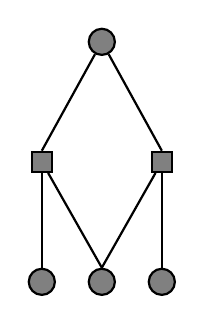
\begin{tikzpicture}
\def \depth{0.6in}; %vertical gap between nodes/levels
\def \gap{0.3in}; %Horizontal gap between nodes
\def \gapA{0.15in}; %Encoder Width
\def \textoffs{0.12in}; %Offset for writing text above a node
\def\nodewidth{0.1in};
\tikzstyle{check} = [rectangle, draw, text centered, thick, fill=gray,
                          minimum height=\nodewidth, minimum width=\nodewidth]
\tikzstyle{bit} = [circle, draw, text centered, thick, fill=gray,
                          radius=0.5*\nodewidth]
                          
\def \fsize{\normalsize}; %Defining a generic font size to be adjusted depending on the scaling
\def \dotsize{\Huge}; %Defining a generic font size to be adjusted depending on the scaling


\node [bit](b1) at (0,0) {} ;

%Level 2
\node[check] (c21) at ([xshift=-\gap,yshift=-\depth]b1) {};
\node[check] (c22) at ([xshift=+\gap,yshift=-\depth]b1) {};

%Lines form level 1-level 2
\draw[thick](b1)--(c21.north);
\draw[thick](b1)--(c22.north);

%Level 3
\node[bit] (b31) at ([xshift=0,yshift=-\depth]c21) {};
\node[bit] (b32) at ([xshift=+\gap,yshift=-\depth]c21) {};
\node[bit] (b33) at ([xshift=0,yshift=-\depth]c22) {};

%Lines form level 2-level 3
\draw[thick](c21)--(b31.north);
\draw[thick](c21)--(b32.north);
\draw[thick](c22)--(b33.north);
\draw[thick](c22)--(b32.north);

\end{tikzpicture}}
\\$O(1/n)$
\end{center}
\end{column}

\begin{column}{0.33\textwidth}
\begin{center}
\scalebox{0.5}{\input{./Figures/compGraph3.tex}}
\\$O(1/n^2)$
\end{center}
\end{column}

\end{columns}
\begin{block}{}
In the limit of large block lengths a computation graph of depth-$l$ looks like a tree w.h.p
\end{block}
\end{frame}
%--------------------------------------------------------------------------------------
\begin{frame}{Analysis of the message passing decoder}
\begin{block}{Computation Tree Ensemble-$\mathcal{T}_{l}(\lambda,\rho)$}
Ensemble of bipartite trees of depth $l$ rooted in a variable node (VN) where
\begin{itemize}
\item Root node has $i$ children(CN's) with probability $L_i$
\item Each VN has $i$ children(CN's) with probability $\lambda_i$
\item Each CN has $i$ children(VN's) with probability $\rho_i$
\end{itemize}
\end{block}
\end{frame}
%--------------------------------------------------------------------------------------
\begin{frame}{Analysis of the message passing decoder}
$\lambda(x)=x^2,\rho(x)=\rho_4 x^3+\rho_5 x^4$ 
\begin{columns}
\only<1,4>{
\begin{column}{0.33\textwidth}
\begin{center}
\scalebox{0.65}{
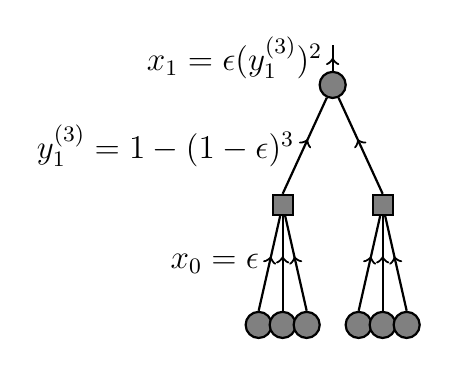
\begin{tikzpicture}
\def \depth{0.6in}; %vertical gap between nodes/levels
\def \gap{0.25in}; %Horizontal gap between nodes
\def \gapA{0.12in}; %Encoder Width
\def \textoffs{0.18in}; %Offset for writing text above a node
\def\nodewidth{0.1in};
\tikzstyle{check} = [rectangle, draw, text centered, thick, fill=gray,
                          minimum height=\nodewidth, minimum width=\nodewidth]
\tikzstyle{bit} = [circle, draw, text centered, thick, fill=gray,
                          radius=0.5*\nodewidth]
                          
\def \fsize{\large}; %Defining a generic font size to be adjusted depending on the scaling
\def \dotsize{\Huge}; %Defining a generic font size to be adjusted depending on the scaling


\node [bit](b1) at (0,0) {} ;
\begin{scope}[thick,decoration={
    markings,
    mark=at position 0.5 with {\arrow{>}}}
    ] 
\draw[postaction={decorate}](b1)--+(0,0.2in)node[midway,left]{\fsize{$x_{1}=\epsilon (y_1^{(3)})^2$}};
\end{scope}


%Level 2
\node[check] (c21) at ([xshift=-\gap,yshift=-\depth]b1) {};
\node[check] (c22) at ([xshift=+\gap,yshift=-\depth]b1) {};

%Lines form level 1-level 2
\begin{scope}[thick,decoration={
    markings,
    mark=at position 0.5 with {\arrow{<}}}
    ] 
\draw[postaction={decorate}](b1)--(c21.north)node[midway,left,align=left]{\fsize{$y_{1}^{(3)}=1-(1-\epsilon)^3$}};
%\draw[postaction={decorate}](b1)--(c21.north)node[midway,left,align=left]{\fsize{$y_{1}^{(3)}=$}\\ \fsize{$1-(1-\epsilon)^3$}};
\draw[postaction={decorate}](b1)--(c22.north);
\end{scope}
%    \draw[postaction={decorate}] (-4,2)--(-4,0);
%\draw[thick](b1)--(c21.north);
%\draw[thick](b1)--(c22.north);

%Level 3
\node[bit] (b31) at ([xshift=-\gapA,yshift=-\depth]c21) {};
\node[bit] (b32) at ([xshift=0,yshift=-\depth]c21) {};
\node[bit] (b33) at ([xshift=+\gapA,yshift=-\depth]c21) {};
\node[bit] (b34) at ([xshift=-\gapA,yshift=-\depth]c22) {};
\node[bit] (b35) at ([xshift=0,yshift=-\depth]c22) {};
\node[bit] (b36) at ([xshift=+\gapA,yshift=-\depth]c22) {};

%Lines form level 2-level 3
\begin{scope}[thick, decoration={
    markings,
    mark=at position 0.5 with {\arrow{<}}}
    ] 
\draw[postaction={decorate}](c21)--(b31.north)node[midway,left]{\fsize{$x_{0}=\epsilon$}};
\draw[postaction={decorate}](c21)--(b32.north);
\draw[postaction={decorate}](c21)--(b33.north); 
\draw[postaction={decorate}](c22)--(b34.north);
\draw[postaction={decorate}](c22)--(b35.north);
\draw[postaction={decorate}](c22)--(b36.north); 
\end{scope}
%\draw[thick](c21)--(b32.north);
%\draw[thick](c21)--(b33.north);
%\draw[thick](c22)--(b34.north);
%\draw[thick](c22)--(b35.north);
%\draw[thick](c22)--(b36.north); 



\end{tikzpicture}}
\\ \scriptsize{$P(T)=\rho_4^2$}
%\\ \scriptsize{$P(T\in\mathcal{T}_1(\lambda,\rho))=\rho_4^2$}
\end{center}
\end{column}
}
\only<2,4>{
\begin{column}{0.33\textwidth}
\begin{center}
\scalebox{0.65}{\input{./Figures/compTree2.tex}}
\\ \scriptsize{$P(T)=2\rho_4\rho_5$}
%\\ \scriptsize{$P(T\in\mathcal{T}_1(\lambda,\rho))=2\rho_4\rho_5$}
\end{center}
\end{column}
}
\only<3,4>{
\begin{column}{0.3\textwidth}
\begin{center}
\scalebox{0.65}{\input{./Figures/compTree3.tex}}
\\ \scriptsize{$P(T)=\rho_5^2$}
%\\ \scriptsize{$P(T\in\mathcal{T}_1(\lambda,\rho))=\rho_5^2$}
\end{center}
\end{column}
}
\end{columns}
\only<4->{
\begin{block}{}
\begin{eqnarray*}
\mathbb{E}_{\text{LDPC}(\lambda,\rho)}[x_1]&=&\sum\limits_{T\in\mathcal{T}_{1}(\lambda,\rho)}P(T)*x_1(T,\epsilon)\\
&=&\epsilon(\rho_4 y_1^{(3)}+\rho_5 y_1^{(4)})^2\\
&=&\epsilon(1-\rho_4 (1-\epsilon)^{3}-\rho_5 (1-\epsilon)^{4})^2\\
&=&\epsilon\lambda\left(1-\rho(1-\epsilon)\right)
%&=&\epsilon(1-\rho(1-\epsilon))^2\\
\end{eqnarray*}
\end{block}
}
\end{frame}
%---------------------------------------------------------------------------------------------------------------------------
\begin{frame}{Density evolution}
\begin{columns}
\begin{column}{0.5\textwidth}
\begin{centering}
\scalebox{0.6}{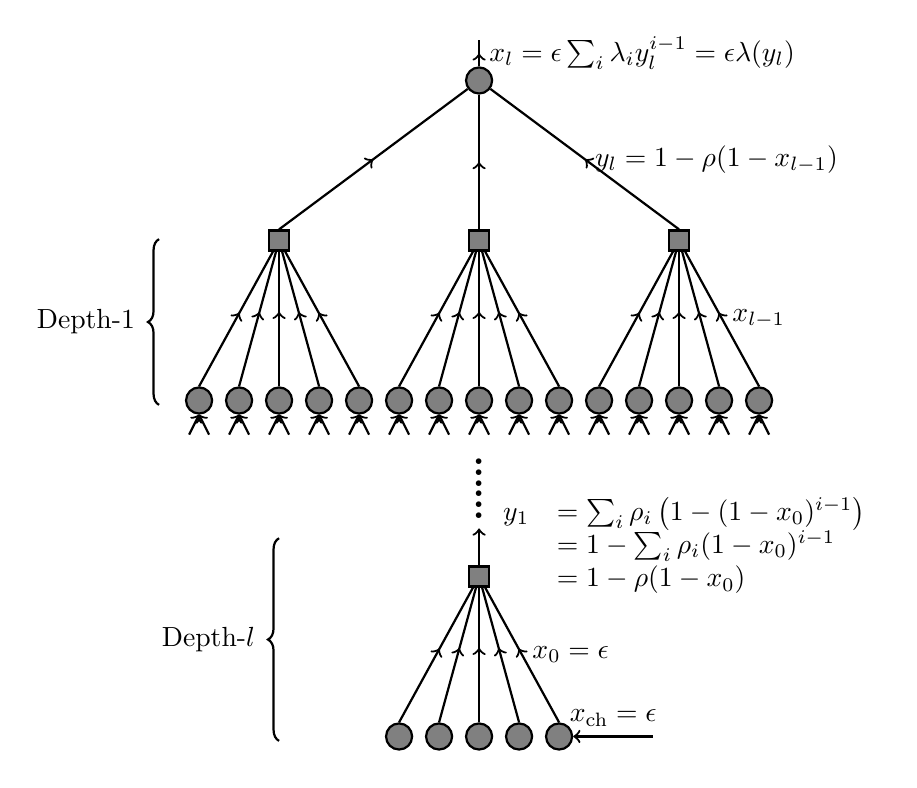
\begin{tikzpicture}
\def \depth{0.8in}; %Encoder Length
\def \gap{1in}; %Encoder Width
\def \gapA{0.2in}; %Encoder Width
\def\nodewidth{0.1in};
\tikzstyle{check} = [rectangle, draw, text centered, thick,fill=gray,
                          minimum height=\nodewidth, minimum width=\nodewidth]
\tikzstyle{bit} = [circle, draw, text centered, thick,fill=gray,
                          radius=0.5*\nodewidth]

\def \fsize{\normalsize}; %Defining a generic font size to be adjusted depending on the scaling
\def \dotsize{\Huge}; %Defining a generic font size to be adjusted depending on the scaling

\node [bit](b1) at (0,0) {} ;
%\node() at ([yshift=0.12in]b1) {$x_{\text{DE}}^{(l)}=\epsilon \sum_{i} \lambda y_l^{i-1}$ };

%Level 2
\node[check] (c21) at ([xshift=-\gap,yshift=-\depth]b1) {};
\node[check] (c22) at ([yshift=-\depth]b1) {};
\node[check] (c23) at ([xshift=+\gap,yshift=-\depth]b1) {};

%Lines form level 1-level 2
\begin{scope}[thick,decoration={
    markings,
    mark=at position 0.5 with {\arrow{>}}}
    ]
\draw[postaction={decorate}] (b1)--+(0,+0.2in)node[midway,right]{$x_{l}=\epsilon \sum_{i} \lambda_i y_l^{i-1} = \epsilon \lambda(y_l)$ };
\draw[postaction={decorate}](c21.north)--(b1);
\draw[postaction={decorate}](c22)--(b1);
\draw[postaction={decorate}](c23.north)--(b1)node[midway,right]{$y_{l}=1-\rho(1- x_{l-1})$};
\end{scope}

%Level 3
\node[bit] (b31) at ([xshift=-2*\gapA,yshift=-\depth]c21) {};
\node[bit] (b32) at ([xshift=-\gapA,yshift=-\depth]c21) {};
\node[bit] (b33) at ([yshift=-\depth]c21) {};
\node[bit] (b34) at ([xshift=+\gapA,yshift=-\depth]c21) {};
\node[bit] (b35) at ([xshift=2*\gapA,yshift=-\depth]c21) {};

\node[bit] (b36) at ([xshift=-2*\gapA,yshift=-\depth]c22) {};
\node[bit] (b37) at ([xshift=-\gapA,yshift=-\depth]c22) {};
\node[bit] (b38) at ([yshift=-\depth]c22) {};
\node[bit] (b39) at ([xshift=+\gapA,yshift=-\depth]c22) {};
\node[bit] (b310) at ([xshift=2*\gapA,yshift=-\depth]c22) {};

\node[bit] (b311) at ([xshift=-2*\gapA,yshift=-\depth]c23) {};
\node[bit] (b312) at ([xshift=-\gapA,yshift=-\depth]c23) {};
\node[bit] (b313) at ([yshift=-\depth]c23) {};
\node[bit] (b314) at ([xshift=+\gapA,yshift=-\depth]c23) {};
\node[bit] (b315) at ([xshift=2*\gapA,yshift=-\depth]c23) {};


%Lines form level 2-level 3
\begin{scope}[thick,decoration={
    markings,
    mark=at position 0.5 with {\arrow{<}}}
    ]
\draw[postaction={decorate}](c21)--(b31.north);
\draw[postaction={decorate}](c21)--(b32.north);
\draw[postaction={decorate}](c21)--(b33.north);
\draw[postaction={decorate}](c21)--(b34.north);
\draw[postaction={decorate}](c21)--(b35.north);

\draw[postaction={decorate}](c22)--(b36.north);
\draw[postaction={decorate}](c22)--(b37.north);
\draw[postaction={decorate}](c22)--(b38.north);
\draw[postaction={decorate}](c22)--(b39.north);
\draw[postaction={decorate}](c22)--(b310.north);

\draw[postaction={decorate}](c23)--(b311.north);
\draw[postaction={decorate}](c23)--(b312.north);
\draw[postaction={decorate}](c23)--(b313.north);
\draw[postaction={decorate}](c23)--(b314.north);
\draw[postaction={decorate}](c23)--(b315.north)node[midway,right]{$x_{l-1}$};%=\epsilon \sum_i \lmb_i y_l^{i-1}  $};
\end{scope}


\node(brace11) at ([xshift=-0.6in]c21.north){};
\node(brace12) at ([xshift=-0.6in]b33.south){};
\draw [decorate,thick,decoration={brace,amplitude=4pt,mirror}](brace11) -- (brace12) node [black,midway,left,xshift=-5pt]{\fsize Depth-$1$};

 \node (dots1) at ([yshift=-0.4*\depth]b38){\dotsize $\vdots$};
\node (dots2) at ([yshift=-0.6*\depth]b38){\dotsize $\vdots$};


%Lines form level 3-level 4
\def \offsx{0.05in};
\def \offsy{0.1in};
\draw[->,thick](b31.south)+(-\offsx,-\offsy)--(b31.south); \draw[->,thick](b31.south)+(\offsx,-\offsy)--(b31.south);
\draw[->,thick](b32.south)+(-\offsx,-\offsy)--(b32.south); \draw[->,thick](b32.south)+(\offsx,-\offsy)--(b32.south);
\draw[->,thick](b33.south)+(-\offsx,-\offsy)--(b33.south); \draw[->,thick](b33.south)+(\offsx,-\offsy)--(b33.south);
\draw[->,thick](b34.south)+(-\offsx,-\offsy)--(b34.south); \draw[->,thick](b34.south)+(\offsx,-\offsy)--(b34.south);
\draw[->,thick](b35.south)+(-\offsx,-\offsy)--(b35.south); \draw[->,thick](b35.south)+(\offsx,-\offsy)--(b35.south);
\draw[->,thick](b36.south)+(-\offsx,-\offsy)--(b36.south); \draw[->,thick](b36.south)+(\offsx,-\offsy)--(b36.south);
\draw[->,thick](b37.south)+(-\offsx,-\offsy)--(b37.south); \draw[->,thick](b37.south)+(\offsx,-\offsy)--(b37.south);
\draw[->,thick](b38.south)+(-\offsx,-\offsy)--(b38.south); \draw[->,thick](b38.south)+(\offsx,-\offsy)--(b38.south);
\draw[->,thick](b39.south)+(-\offsx,-\offsy)--(b39.south); \draw[->,thick](b39.south)+(\offsx,-\offsy)--(b39.south);
\draw[->,thick](b310.south)+(-\offsx,-\offsy)--(b310.south); \draw[->,thick](b310.south)+(\offsx,-\offsy)--(b310.south);
\draw[->,thick](b311.south)+(-\offsx,-\offsy)--(b311.south); \draw[->,thick](b311.south)+(\offsx,-\offsy)--(b311.south);
\draw[->,thick](b312.south)+(-\offsx,-\offsy)--(b312.south); \draw[->,thick](b312.south)+(\offsx,-\offsy)--(b312.south);
\draw[->,thick](b313.south)+(-\offsx,-\offsy)--(b313.south); \draw[->,thick](b313.south)+(\offsx,-\offsy)--(b313.south);
\draw[->,thick](b314.south)+(-\offsx,-\offsy)--(b314.south); \draw[->,thick](b314.south)+(\offsx,-\offsy)--(b314.south);
\draw[->,thick](b315.south)+(-\offsx,-\offsy)--(b315.south); \draw[->,thick](b315.south)+(\offsx,-\offsy)--(b315.south);

%Level l
\node[check] (cL1) at ([yshift=-0.5*\depth]dots2) {};

\draw[<-,thick](dots2.south)--(cL1.north)node[midway,right]{$\begin{array}{ll}y_{1}& = \sum_i \rho_i \left(1-(1-x_0)^{i-1} \right)\\
& = 1-\sum_i \rho_i (1-x_0)^{i-1} \\ & = 1-\rho(1-x_{0})\end{array}$};;

%Level l+1
\node[bit] (bl1) at ([xshift=-2*\gapA,yshift=-\depth]cL1) {};
\node[bit] (bl2) at ([xshift=-\gapA,yshift=-\depth]cL1) {};
\node[bit] (bl3) at ([yshift=-\depth]cL1) {};
\node[bit] (bl4) at ([xshift=\gapA,yshift=-\depth]cL1) {};
\node[bit] (bl5) at ([xshift=2*\gapA,yshift=-\depth]cL1) {};


%Lines form level l-level l+1
\begin{scope}[thick,decoration={
    markings,
    mark=at position 0.5 with {\arrow{<}}}
    ]
\draw[postaction={decorate}](cL1)--(bl1.north);
\draw[postaction={decorate}](cL1)--(bl2.north);
\draw[postaction={decorate}](cL1)--(bl3.north);
\draw[postaction={decorate}](cL1)--(bl4.north);
\draw[postaction={decorate}](cL1)--(bl5.north)node[midway,right]{$x_{0}=\epsilon$};
\end{scope}

\draw[<-,thick](bl5.east)--+(2*\gapA,0)node[midway,above]{$x_{\text{ch}}=\epsilon$};


\node(lbrace1) at ([xshift=-1in]dots2.south){};
\node(lbrace2) at ([xshift=-1in]bl3.south){};
\draw [decorate,thick,decoration={brace,amplitude=4pt,mirror}](lbrace1) -- (lbrace2) node [black,midway,left,xshift=-5pt]{\fsize Depth-$l$};


%\draw[<-,thick](enc)-- +(-\ext,0) node[midway,above]{\fsize $m_1,\ldots,m_l$};
%\draw[<-,thick](enc)--(chan)node[midway,above]{\fsize $c_1,\ldots,c_l$}node[midway,below]{\fsize $c_i\in \mathbb{F}_p$};
%\draw[<-,thick](chan)--(dec)node[midway,above]{\fsize $r_1,\ldots,r_l$}node[midway,below]{\fsize $r_i\in \mathbb{F}_p$};;
%
%\draw[<-,thick](chan)--+(0,\extB) node[above] {\fsize $e_1,\ldots,e_l$};
%\draw[<-,thick](dec)--+(\ext,0)node[midway,above]{\fsize  $\hat{m_1},\ldots,\hat{m_l}$};
%
\end{tikzpicture} }
\end{centering}
\end{column}

\begin{column}{0.5\textwidth}
\only<2->{
\begin{block}{Recursion}
\begin{eqnarray*}
  x_0 &=& \epsilon \\
  y_l &=& 1-\rho(1-x_{l-1}) \\
  x_l &=& \epsilon \lambda(y_l)\\
  x_l &=& \epsilon \lambda(1-\rho(1-x_{l-1})) 
\end{eqnarray*}
\end{block}
}
\end{column}
\end{columns}
\end{frame}
%--------------------------------------------------------------------------------------
\begin{frame}{Density evolution}
\begin{block}{Recursion}
\begin{eqnarray*}
  y_0 &=& 1 \\
  x_l &=& \epsilon \lambda(y_{l-1}) \\
  y_l &=& 1-\rho(1-x_l) \\
  x_l &=& \epsilon \lambda(1-\rho(1-x_{l-1})) = f(\epsilon,x_{l-1})
\end{eqnarray*}
\end{block}

\begin{block}{Convergence condition}
\[
f(\epsilon,x) < x, \ x \in (0,\epsilon]
\]
\end{block}
\begin{block}{Threshold of $(\lambda,\rho)$ pair}
The threshold $\epsilon^{\text{BP}}(\lambda,\rho)$ is defined as
\[
\epsilon^{\text{BP}}(\lambda,\rho) = \sup \{\epsilon \in [0,1]: x_l \rightarrow 0 \ \text{as} \ l \rightarrow \infty \}
\]
\end{block}
\end{frame}
%--------------------------------------------------------------------------------------
\begin{frame}{Exit Charts}
\begin{block}{Node functions}
\begin{itemize}
\item Var node function: $v_{\epsilon}(x) = \epsilon \lambda(x)$
\item Check node function: $c(x) = 1- \rho(1-x)$
\end{itemize}
\end{block}
\begin{columns}
\begin{column}{0.47\textwidth}
\begin{center}
\scalebox{0.35}{% This file was created by matlab2tikz v0.4.7 running on MATLAB 7.14.
% Copyright (c) 2008--2014, Nico Schlömer <nico.schloemer@gmail.com>
% All rights reserved.
% Minimal pgfplots version: 1.3
% 
% The latest updates can be retrieved from
%   http://www.mathworks.com/matlabcentral/fileexchange/22022-matlab2tikz
% where you can also make suggestions and rate matlab2tikz.
% 
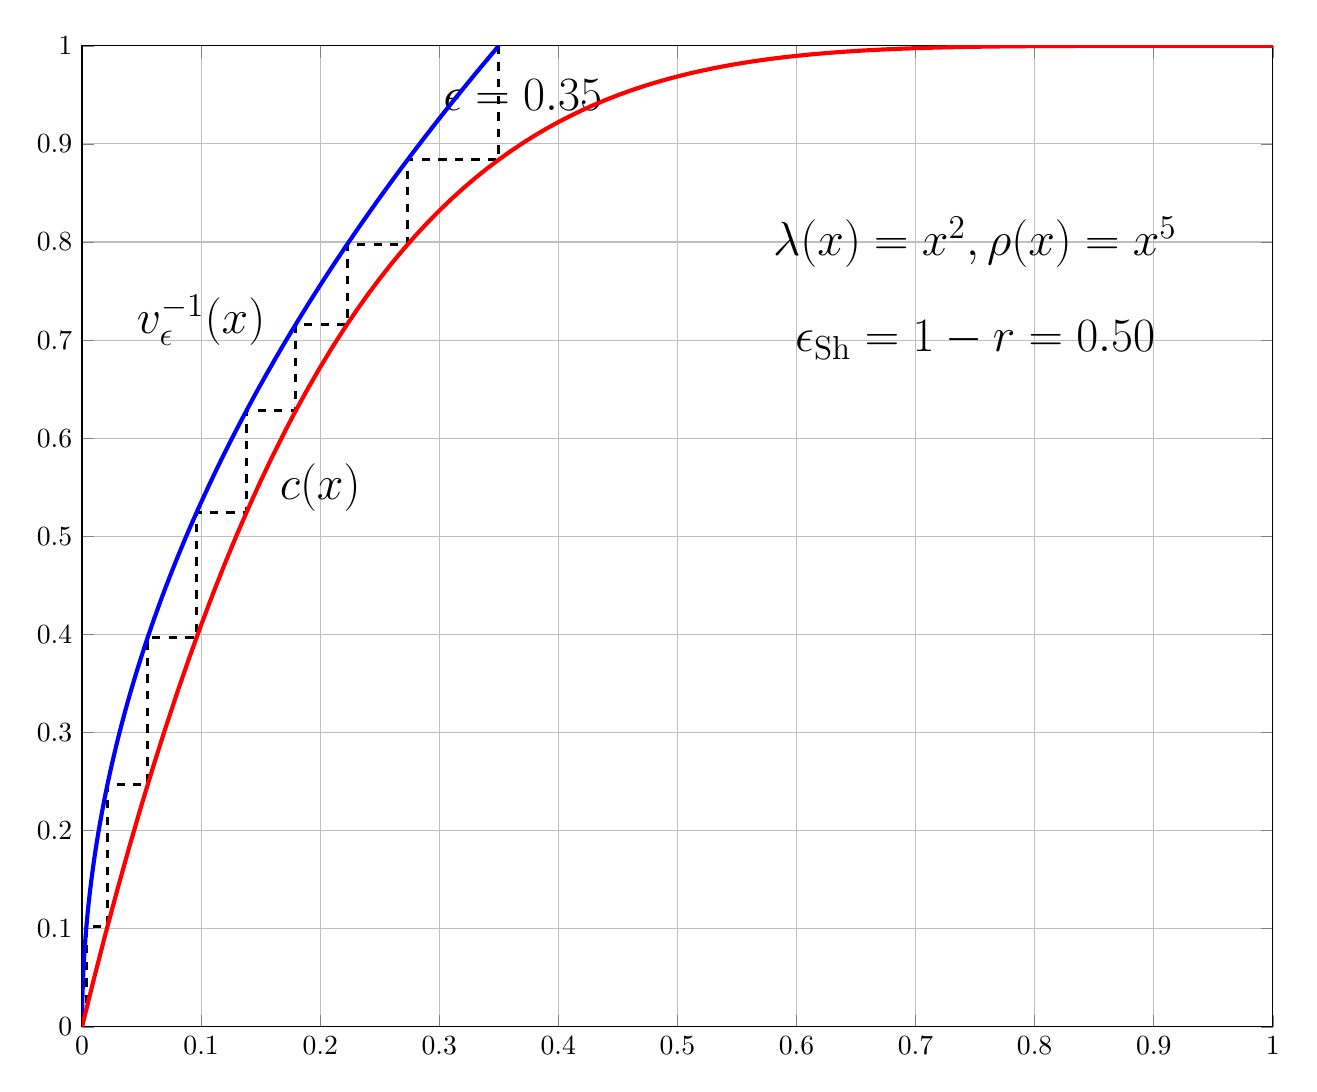
\begin{tikzpicture}
\def\fsize{\LARGE}
\begin{axis}[%
width=5.95380358705162in,
height=4.90490244969379in,
scale only axis,
xmin=0,
xmax=1,
xmajorgrids,
ymin=0,
ymax=1,
ymajorgrids
]
\node at (axis cs:0.2,0.55) {\fsize{$c(x)$}};
\node at (axis cs:0.1,0.72) {\fsize{$v_{\epsilon}^{-1}(x)$}};
\node at (axis cs:0.37,0.95) {\fsize{$\epsilon=0.35$}};

\node at (axis cs:0.75,0.8){\fsize{$\lambda(x)=x^2,\rho(x)=x^{5}$}};%\sum_{i=1}^{N}\binom{\alpha}{i}(-1)^{i-1}x^i$}};
\node at (axis cs:0.75,0.7){\fsize{$\epsilon_{\text{Sh}}=1-r=0.50 $}};
%\node at (axis cs:0.75,0.8){\fsize{$\rho(x)=x^{10},\alpha=0.1,N=50.$}};



\addplot [color=black,dashed,line width=1.0pt]
  table[row sep=crcr]{0.35	1\\
0.350000  0.883971 \\ 
0.273492  0.883971 \\ 
0.273492  0.797603 \\ 
0.222660  0.797603 \\ 
0.222660  0.716172 \\ 
0.179516  0.716172 \\ 
0.179516  0.628164 \\ 
0.138107  0.628164 \\ 
0.138107  0.524372 \\ 
0.096238  0.524372 \\ 
0.096238  0.397065 \\ 
0.055181  0.397065 \\ 
0.055181  0.247091 \\ 
0.021369  0.247091 \\ 
0.021369  0.102375 \\ 
0.003668  0.102375 \\ 
0.003668  0.018207 \\ 
0.000116  0.018207 \\ 
0.000116  0.000580 \\ 
0.000000  0.000580 \\ 
};
  
\addplot [color=blue,solid,line width=1.5pt]
  table[row sep=crcr]{0	0\\
3.5e-05	0.01\\
0.00014	0.02\\
0.000315	0.03\\
0.00056	0.04\\
0.000875	0.05\\
0.00126	0.06\\
0.001715	0.07\\
0.00224	0.08\\
0.002835	0.09\\
0.0035	0.1\\
0.004235	0.11\\
0.00504	0.12\\
0.005915	0.13\\
0.00686	0.14\\
0.007875	0.15\\
0.00896	0.16\\
0.010115	0.17\\
0.01134	0.18\\
0.012635	0.19\\
0.014	0.2\\
0.015435	0.21\\
0.01694	0.22\\
0.018515	0.23\\
0.02016	0.24\\
0.021875	0.25\\
0.02366	0.26\\
0.025515	0.27\\
0.02744	0.28\\
0.029435	0.29\\
0.0315	0.3\\
0.033635	0.31\\
0.03584	0.32\\
0.038115	0.33\\
0.04046	0.34\\
0.042875	0.35\\
0.04536	0.36\\
0.047915	0.37\\
0.05054	0.38\\
0.053235	0.39\\
0.056	0.4\\
0.058835	0.41\\
0.06174	0.42\\
0.064715	0.43\\
0.06776	0.44\\
0.070875	0.45\\
0.07406	0.46\\
0.077315	0.47\\
0.08064	0.48\\
0.084035	0.49\\
0.0875	0.5\\
0.091035	0.51\\
0.09464	0.52\\
0.098315	0.53\\
0.10206	0.54\\
0.105875	0.55\\
0.10976	0.56\\
0.113715	0.57\\
0.11774	0.58\\
0.121835	0.59\\
0.126	0.6\\
0.130235	0.61\\
0.13454	0.62\\
0.138915	0.63\\
0.14336	0.64\\
0.147875	0.65\\
0.15246	0.66\\
0.157115	0.67\\
0.16184	0.68\\
0.166635	0.69\\
0.1715	0.7\\
0.176435	0.71\\
0.18144	0.72\\
0.186515	0.73\\
0.19166	0.74\\
0.196875	0.75\\
0.20216	0.76\\
0.207515	0.77\\
0.21294	0.78\\
0.218435	0.79\\
0.224	0.8\\
0.229635	0.81\\
0.23534	0.82\\
0.241115	0.83\\
0.24696	0.84\\
0.252875	0.85\\
0.25886	0.86\\
0.264915	0.87\\
0.27104	0.88\\
0.277235	0.89\\
0.2835	0.9\\
0.289835	0.91\\
0.29624	0.92\\
0.302715	0.93\\
0.30926	0.94\\
0.315875	0.95\\
0.32256	0.96\\
0.329315	0.97\\
0.33614	0.98\\
0.343035	0.99\\
0.35	1\\
};
\addplot [color=red,solid,line width=1.5pt]
  table[row sep=crcr]{0	0\\
0.01	0.0490099501000001\\
0.02	0.0960792032000002\\
0.03	0.1412659743\\
0.04	0.1846273024\\
0.05	0.2262190625\\
0.06	0.2660959776\\
0.07	0.3043116307\\
0.08	0.3409184768\\
0.09	0.3759678549\\
0.1	0.40951\\
0.11	0.4415940551\\
0.12	0.4722680832\\
0.13	0.5015790793\\
0.14	0.5295729824\\
0.15	0.5562946875\\
0.16	0.5817880576\\
0.17	0.6060959357\\
0.18	0.6292601568\\
0.19	0.6513215599\\
0.2	0.67232\\
0.21	0.6922943601\\
0.22	0.7112825632\\
0.23	0.7293215843\\
0.24	0.7464474624\\
0.25	0.7626953125\\
0.26	0.7780993376\\
0.27	0.7926928407\\
0.28	0.8065082368\\
0.29	0.8195770649\\
0.3	0.83193\\
0.31	0.8435968651\\
0.32	0.8546066432\\
0.33	0.8649874893\\
0.34	0.8747667424\\
0.35	0.8839709375\\
0.36	0.8926258176\\
0.37	0.9007563457\\
0.38	0.9083867168\\
0.39	0.9155403699\\
0.4	0.92224\\
0.41	0.9285075701\\
0.42	0.9343643232\\
0.43	0.9398307943\\
0.44	0.9449268224\\
0.45	0.9496715625\\
0.46	0.9540834976\\
0.47	0.9581804507\\
0.48	0.9619795968\\
0.49	0.9654974749\\
0.5	0.96875\\
0.51	0.9717524751\\
0.52	0.9745196032\\
0.53	0.9770654993\\
0.54	0.9794037024\\
0.55	0.9815471875\\
0.56	0.9835083776\\
0.57	0.9852991557\\
0.58	0.9869308768\\
0.59	0.9884143799\\
0.6	0.98976\\
0.61	0.9909775801\\
0.62	0.9920764832\\
0.63	0.9930656043\\
0.64	0.9939533824\\
0.65	0.9947478125\\
0.66	0.9954564576\\
0.67	0.9960864607\\
0.68	0.9966445568\\
0.69	0.9971370849\\
0.7	0.99757\\
0.71	0.9979488851\\
0.72	0.9982789632\\
0.73	0.9985651093\\
0.74	0.9988118624\\
0.75	0.9990234375\\
0.76	0.9992037376\\
0.77	0.9993563657\\
0.78	0.9994846368\\
0.79	0.9995915899\\
0.8	0.99968\\
0.81	0.9997523901\\
0.82	0.9998110432\\
0.83	0.9998580143\\
0.84	0.9998951424\\
0.85	0.9999240625\\
0.86	0.9999462176\\
0.87	0.9999628707\\
0.88	0.9999751168\\
0.89	0.9999838949\\
0.9	0.99999\\
0.91	0.9999940951\\
0.92	0.9999967232\\
0.93	0.9999983193\\
0.94	0.9999992224\\
0.95	0.9999996875\\
0.96	0.9999998976\\
0.97	0.9999999757\\
0.98	0.9999999968\\
0.99	0.9999999999\\
1	1\\
};
\end{axis}
\end{tikzpicture}%}
\end{center}
\end{column}

\begin{column}{0.47\textwidth}
\begin{center}
\scalebox{0.35}{% This file was created by matlab2tikz v0.4.7 running on MATLAB 7.14.
% Copyright (c) 2008--2014, Nico Schlömer <nico.schloemer@gmail.com>
% All rights reserved.
% Minimal pgfplots version: 1.3
% 
% The latest updates can be retrieved from
%   http://www.mathworks.com/matlabcentral/fileexchange/22022-matlab2tikz
% where you can also make suggestions and rate matlab2tikz.
% 
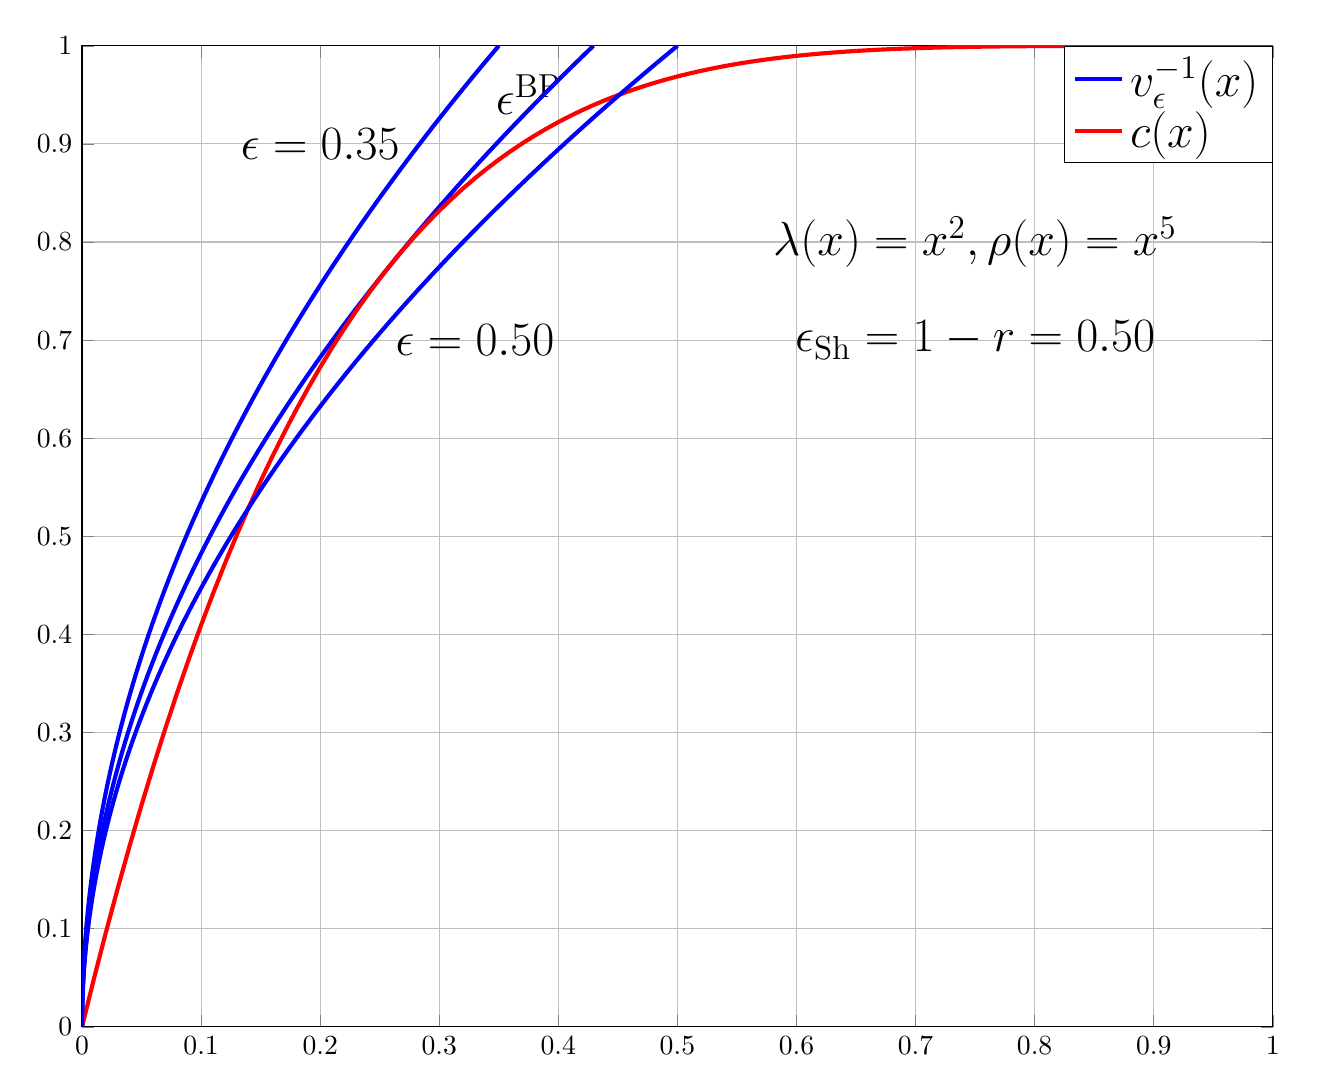
\begin{tikzpicture}
\def\fsize{\LARGE}
\begin{axis}[%
width=5.95380358705162in,
height=4.90490244969379in,
scale only axis,
xmin=0,
xmax=1,
xmajorgrids,
ymin=0,
ymax=1,
legend style={at={(1,1)},anchor=north east,draw=black,fill=white,legend cell align=left,font=\LARGE},
ymajorgrids
]
\node at (axis cs:0.33,0.7){\LARGE{$\epsilon=0.50$}};
\node at (axis cs:0.2,0.9){\LARGE{$\epsilon=0.35$}};
\node at (axis cs:0.375,0.95){\LARGE{$\epsilon^{\text{BP}}$}};

\node at (axis cs:0.75,0.8){\fsize{$\lambda(x)=x^2,\rho(x)=x^{5}$}};%\sum_{i=1}^{N}\binom{\alpha}{i}(-1)^{i-1}x^i$}};
\node at (axis cs:0.75,0.7){\fsize{$\epsilon_{\text{Sh}}=1-r=0.50 $}};

\addlegendentry{\LARGE{$v_{\epsilon}^{-1}(x)$}};
\addplot [color=blue,solid,line width=1.5pt]
  table[row sep=crcr]{0	0\\
4.2944e-05	0.01\\
0.000171776	0.02\\
0.000386496	0.03\\
0.000687104	0.04\\
0.0010736	0.05\\
0.001545984	0.06\\
0.002104256	0.07\\
0.002748416	0.08\\
0.003478464	0.09\\
0.0042944	0.1\\
0.005196224	0.11\\
0.006183936	0.12\\
0.007257536	0.13\\
0.008417024	0.14\\
0.0096624	0.15\\
0.010993664	0.16\\
0.012410816	0.17\\
0.013913856	0.18\\
0.015502784	0.19\\
0.0171776	0.2\\
0.018938304	0.21\\
0.020784896	0.22\\
0.022717376	0.23\\
0.024735744	0.24\\
0.02684	0.25\\
0.029030144	0.26\\
0.031306176	0.27\\
0.033668096	0.28\\
0.036115904	0.29\\
0.0386496	0.3\\
0.041269184	0.31\\
0.043974656	0.32\\
0.046766016	0.33\\
0.049643264	0.34\\
0.0526064	0.35\\
0.055655424	0.36\\
0.058790336	0.37\\
0.062011136	0.38\\
0.065317824	0.39\\
0.0687104	0.4\\
0.072188864	0.41\\
0.075753216	0.42\\
0.079403456	0.43\\
0.083139584	0.44\\
0.0869616	0.45\\
0.090869504	0.46\\
0.094863296	0.47\\
0.098942976	0.48\\
0.103108544	0.49\\
0.10736	0.5\\
0.111697344	0.51\\
0.116120576	0.52\\
0.120629696	0.53\\
0.125224704	0.54\\
0.1299056	0.55\\
0.134672384	0.56\\
0.139525056	0.57\\
0.144463616	0.58\\
0.149488064	0.59\\
0.1545984	0.6\\
0.159794624	0.61\\
0.165076736	0.62\\
0.170444736	0.63\\
0.175898624	0.64\\
0.1814384	0.65\\
0.187064064	0.66\\
0.192775616	0.67\\
0.198573056	0.68\\
0.204456384	0.69\\
0.2104256	0.7\\
0.216480704	0.71\\
0.222621696	0.72\\
0.228848576	0.73\\
0.235161344	0.74\\
0.24156	0.75\\
0.248044544	0.76\\
0.254614976	0.77\\
0.261271296	0.78\\
0.268013504	0.79\\
0.2748416	0.8\\
0.281755584	0.81\\
0.288755456	0.82\\
0.295841216	0.83\\
0.303012864	0.84\\
0.3102704	0.85\\
0.317613824	0.86\\
0.325043136	0.87\\
0.332558336	0.88\\
0.340159424	0.89\\
0.3478464	0.9\\
0.355619264	0.91\\
0.363478016	0.92\\
0.371422656	0.93\\
0.379453184	0.94\\
0.3875696	0.95\\
0.395771904	0.96\\
0.404060096	0.97\\
0.412434176	0.98\\
0.420894144	0.99\\
0.42944	1\\
};

\addlegendentry{\LARGE{$c(x)$}};
\addplot [color=red,solid,line width=1.5pt]
  table[row sep=crcr]{0	0\\
0.01	0.0490099501000001\\
0.02	0.0960792032000002\\
0.03	0.1412659743\\
0.04	0.1846273024\\
0.05	0.2262190625\\
0.06	0.2660959776\\
0.07	0.3043116307\\
0.08	0.3409184768\\
0.09	0.3759678549\\
0.1	0.40951\\
0.11	0.4415940551\\
0.12	0.4722680832\\
0.13	0.5015790793\\
0.14	0.5295729824\\
0.15	0.5562946875\\
0.16	0.5817880576\\
0.17	0.6060959357\\
0.18	0.6292601568\\
0.19	0.6513215599\\
0.2	0.67232\\
0.21	0.6922943601\\
0.22	0.7112825632\\
0.23	0.7293215843\\
0.24	0.7464474624\\
0.25	0.7626953125\\
0.26	0.7780993376\\
0.27	0.7926928407\\
0.28	0.8065082368\\
0.29	0.8195770649\\
0.3	0.83193\\
0.31	0.8435968651\\
0.32	0.8546066432\\
0.33	0.8649874893\\
0.34	0.8747667424\\
0.35	0.8839709375\\
0.36	0.8926258176\\
0.37	0.9007563457\\
0.38	0.9083867168\\
0.39	0.9155403699\\
0.4	0.92224\\
0.41	0.9285075701\\
0.42	0.9343643232\\
0.43	0.9398307943\\
0.44	0.9449268224\\
0.45	0.9496715625\\
0.46	0.9540834976\\
0.47	0.9581804507\\
0.48	0.9619795968\\
0.49	0.9654974749\\
0.5	0.96875\\
0.51	0.9717524751\\
0.52	0.9745196032\\
0.53	0.9770654993\\
0.54	0.9794037024\\
0.55	0.9815471875\\
0.56	0.9835083776\\
0.57	0.9852991557\\
0.58	0.9869308768\\
0.59	0.9884143799\\
0.6	0.98976\\
0.61	0.9909775801\\
0.62	0.9920764832\\
0.63	0.9930656043\\
0.64	0.9939533824\\
0.65	0.9947478125\\
0.66	0.9954564576\\
0.67	0.9960864607\\
0.68	0.9966445568\\
0.69	0.9971370849\\
0.7	0.99757\\
0.71	0.9979488851\\
0.72	0.9982789632\\
0.73	0.9985651093\\
0.74	0.9988118624\\
0.75	0.9990234375\\
0.76	0.9992037376\\
0.77	0.9993563657\\
0.78	0.9994846368\\
0.79	0.9995915899\\
0.8	0.99968\\
0.81	0.9997523901\\
0.82	0.9998110432\\
0.83	0.9998580143\\
0.84	0.9998951424\\
0.85	0.9999240625\\
0.86	0.9999462176\\
0.87	0.9999628707\\
0.88	0.9999751168\\
0.89	0.9999838949\\
0.9	0.99999\\
0.91	0.9999940951\\
0.92	0.9999967232\\
0.93	0.9999983193\\
0.94	0.9999992224\\
0.95	0.9999996875\\
0.96	0.9999998976\\
0.97	0.9999999757\\
0.98	0.9999999968\\
0.99	0.9999999999\\
1	1\\
};

\addplot [color=blue,solid,line width=1.5pt]
  table[row sep=crcr]{0	0\\
3.5e-05	0.01\\
0.00014	0.02\\
0.000315	0.03\\
0.00056	0.04\\
0.000875	0.05\\
0.00126	0.06\\
0.001715	0.07\\
0.00224	0.08\\
0.002835	0.09\\
0.0035	0.1\\
0.004235	0.11\\
0.00504	0.12\\
0.005915	0.13\\
0.00686	0.14\\
0.007875	0.15\\
0.00896	0.16\\
0.010115	0.17\\
0.01134	0.18\\
0.012635	0.19\\
0.014	0.2\\
0.015435	0.21\\
0.01694	0.22\\
0.018515	0.23\\
0.02016	0.24\\
0.021875	0.25\\
0.02366	0.26\\
0.025515	0.27\\
0.02744	0.28\\
0.029435	0.29\\
0.0315	0.3\\
0.033635	0.31\\
0.03584	0.32\\
0.038115	0.33\\
0.04046	0.34\\
0.042875	0.35\\
0.04536	0.36\\
0.047915	0.37\\
0.05054	0.38\\
0.053235	0.39\\
0.056	0.4\\
0.058835	0.41\\
0.06174	0.42\\
0.064715	0.43\\
0.06776	0.44\\
0.070875	0.45\\
0.07406	0.46\\
0.077315	0.47\\
0.08064	0.48\\
0.084035	0.49\\
0.0875	0.5\\
0.091035	0.51\\
0.09464	0.52\\
0.098315	0.53\\
0.10206	0.54\\
0.105875	0.55\\
0.10976	0.56\\
0.113715	0.57\\
0.11774	0.58\\
0.121835	0.59\\
0.126	0.6\\
0.130235	0.61\\
0.13454	0.62\\
0.138915	0.63\\
0.14336	0.64\\
0.147875	0.65\\
0.15246	0.66\\
0.157115	0.67\\
0.16184	0.68\\
0.166635	0.69\\
0.1715	0.7\\
0.176435	0.71\\
0.18144	0.72\\
0.186515	0.73\\
0.19166	0.74\\
0.196875	0.75\\
0.20216	0.76\\
0.207515	0.77\\
0.21294	0.78\\
0.218435	0.79\\
0.224	0.8\\
0.229635	0.81\\
0.23534	0.82\\
0.241115	0.83\\
0.24696	0.84\\
0.252875	0.85\\
0.25886	0.86\\
0.264915	0.87\\
0.27104	0.88\\
0.277235	0.89\\
0.2835	0.9\\
0.289835	0.91\\
0.29624	0.92\\
0.302715	0.93\\
0.30926	0.94\\
0.315875	0.95\\
0.32256	0.96\\
0.329315	0.97\\
0.33614	0.98\\
0.343035	0.99\\
0.35	1\\
};

\addplot [color=blue,solid,line width=1.5pt]
  table[row sep=crcr]{0	0\\
5e-05	0.01\\
0.0002	0.02\\
0.00045	0.03\\
0.0008	0.04\\
0.00125	0.05\\
0.0018	0.06\\
0.00245	0.07\\
0.0032	0.08\\
0.00405	0.09\\
0.005	0.1\\
0.00605	0.11\\
0.0072	0.12\\
0.00845	0.13\\
0.0098	0.14\\
0.01125	0.15\\
0.0128	0.16\\
0.01445	0.17\\
0.0162	0.18\\
0.01805	0.19\\
0.02	0.2\\
0.02205	0.21\\
0.0242	0.22\\
0.02645	0.23\\
0.0288	0.24\\
0.03125	0.25\\
0.0338	0.26\\
0.03645	0.27\\
0.0392	0.28\\
0.04205	0.29\\
0.045	0.3\\
0.04805	0.31\\
0.0512	0.32\\
0.05445	0.33\\
0.0578	0.34\\
0.06125	0.35\\
0.0648	0.36\\
0.06845	0.37\\
0.0722	0.38\\
0.07605	0.39\\
0.08	0.4\\
0.08405	0.41\\
0.0882	0.42\\
0.09245	0.43\\
0.0968	0.44\\
0.10125	0.45\\
0.1058	0.46\\
0.11045	0.47\\
0.1152	0.48\\
0.12005	0.49\\
0.125	0.5\\
0.13005	0.51\\
0.1352	0.52\\
0.14045	0.53\\
0.1458	0.54\\
0.15125	0.55\\
0.1568	0.56\\
0.16245	0.57\\
0.1682	0.58\\
0.17405	0.59\\
0.18	0.6\\
0.18605	0.61\\
0.1922	0.62\\
0.19845	0.63\\
0.2048	0.64\\
0.21125	0.65\\
0.2178	0.66\\
0.22445	0.67\\
0.2312	0.68\\
0.23805	0.69\\
0.245	0.7\\
0.25205	0.71\\
0.2592	0.72\\
0.26645	0.73\\
0.2738	0.74\\
0.28125	0.75\\
0.2888	0.76\\
0.29645	0.77\\
0.3042	0.78\\
0.31205	0.79\\
0.32	0.8\\
0.32805	0.81\\
0.3362	0.82\\
0.34445	0.83\\
0.3528	0.84\\
0.36125	0.85\\
0.3698	0.86\\
0.37845	0.87\\
0.3872	0.88\\
0.39605	0.89\\
0.405	0.9\\
0.41405	0.91\\
0.4232	0.92\\
0.43245	0.93\\
0.4418	0.94\\
0.45125	0.95\\
0.4608	0.96\\
0.47045	0.97\\
0.4802	0.98\\
0.49005	0.99\\
0.5	1\\
};
\end{axis}
\end{tikzpicture}%}
\end{center}

\end{column}

\end{columns}
\end{frame}
%--------------------------------------------------------------------------------------
\begin{frame}{Optimality of EXIT chart matching}
\begin{itemize}
\item Var node function: $v_{\epsilon}(x) = \epsilon \lambda(x)$
\item Check node function: $c(x) = 1- \rho(1-x)$
\end{itemize}
\begin{center}
\scalebox{0.45}{% This file was created by matlab2tikz v0.4.7 running on MATLAB 7.14.
% Copyright (c) 2008--2014, Nico Schlömer <nico.schloemer@gmail.com>
% All rights reserved.
% Minimal pgfplots version: 1.3
% 
% The latest updates can be retrieved from
%   http://www.mathworks.com/matlabcentral/fileexchange/22022-matlab2tikz
% where you can also make suggestions and rate matlab2tikz.
% 
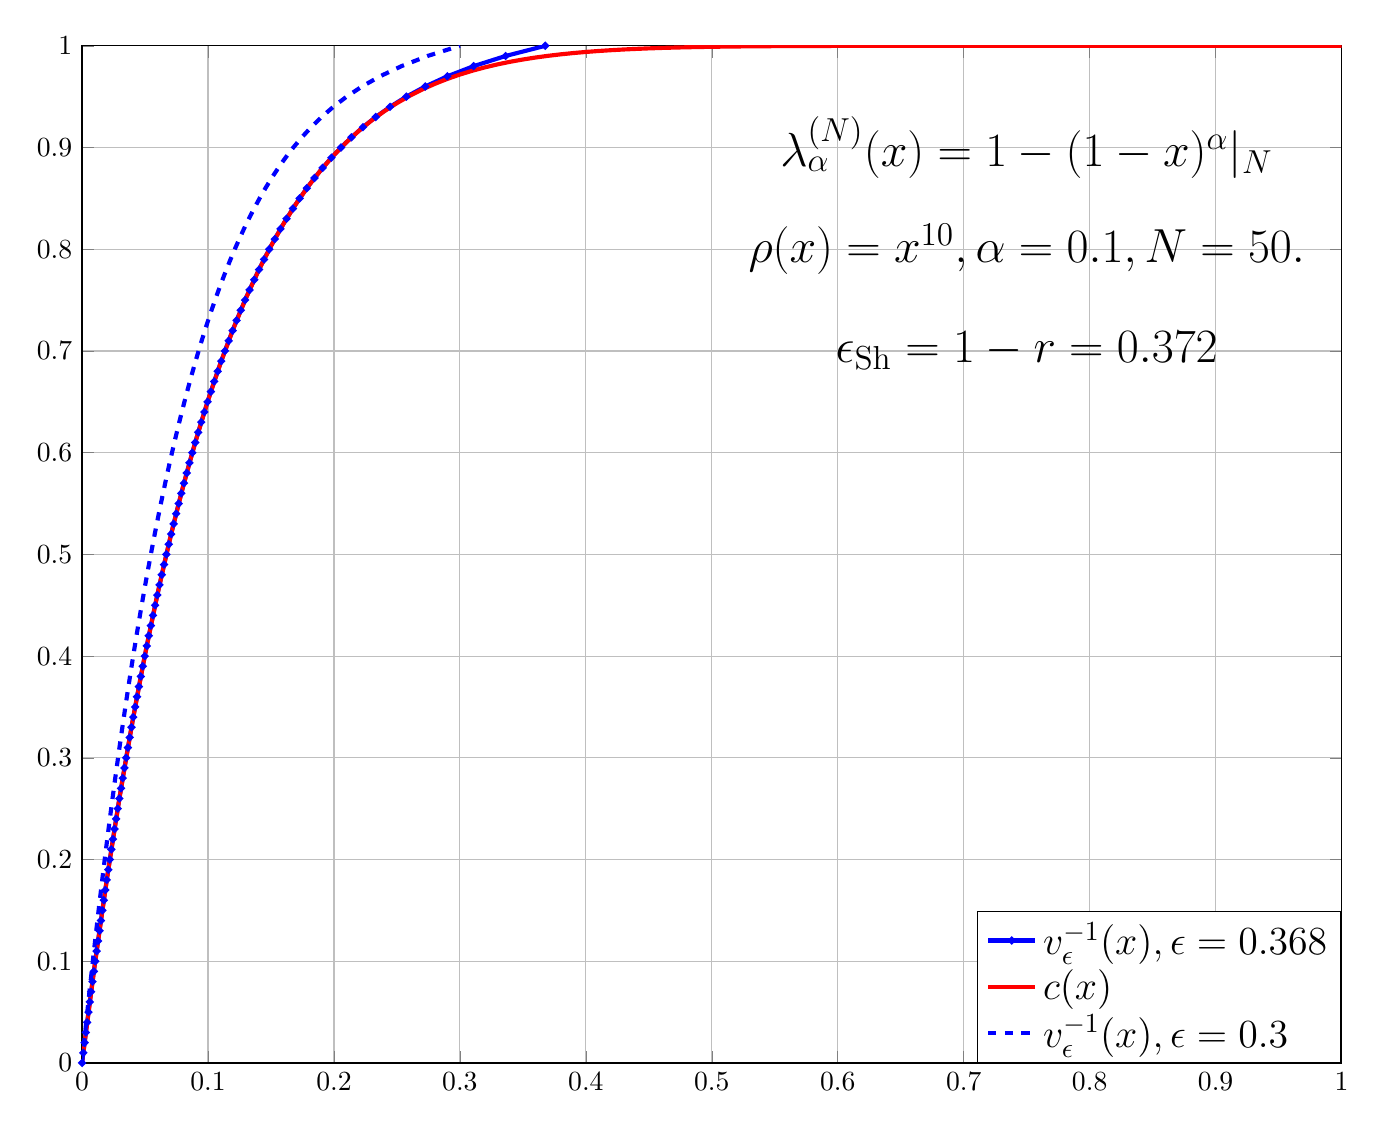
\begin{tikzpicture}
\def \fsize{\LARGE}
\begin{axis}[%
width=6.29770559930009in,
height=5.08572834645669in,
scale only axis,
xmin=0,
xmax=1,
xmajorgrids,
ymin=0,
ymax=1,
legend style={at={(1,0)},anchor=south east,draw=black,fill=white,legend cell align=left,font=\fsize},
ymajorgrids
]

\node at (axis cs:0.75,0.9){\fsize{$\lambda_{\alpha}^{(N)}(x)=1-(1-x)^{\alpha}|_{N}$}};%\sum_{i=1}^{N}\binom{\alpha}{i}(-1)^{i-1}x^i$}};
\node at (axis cs:0.75,0.8){\fsize{$\rho(x)=x^{10},\alpha=0.1,N=50.$}};
\node at (axis cs:0.75,0.7){\fsize{$\epsilon_{\text{Sh}}=1-r=0.372 $}};


\addlegendentry{\Large{$v_{\epsilon}^{-1}(x),\epsilon=0.368$}};
\addplot [color=blue,mark=*,mark size=0.5pt,solid,line width=1.5pt]
  table[row sep=crcr]{0	0\\
0.00100452870824995	0.01\\
0.00201823135843042	0.02\\
0.0030412866381062	0.03\\
0.00407387860214938	0.04\\
0.0051161968918237	0.05\\
0.00616843696522343	0.06\\
0.00723080033978309	0.07\\
0.00830349484762741	0.08\\
0.00938673490458918	0.09\\
0.0104807417937856	0.1\\
0.0115857439647124	0.11\\
0.0127019773488898	0.12\\
0.0138296856931755	0.13\\
0.0149691209119498	0.14\\
0.0161205434594737	0.15\\
0.0172842227238285	0.16\\
0.0184604374439603	0.17\\
0.0196494761514822	0.18\\
0.0208516376390232	0.19\\
0.0220672314570715	0.2\\
0.0232965784414229	0.21\\
0.0245400112735353	0.22\\
0.0257978750762919	0.23\\
0.0270705280479034	0.24\\
0.0283583421369265	0.25\\
0.0296617037616551	0.26\\
0.0309810145774423	0.27\\
0.0323166922958518	0.28\\
0.0336691715599149	0.29\\
0.0350389048801824	0.3\\
0.0364263636367327	0.31\\
0.0378320391528112	0.32\\
0.0392564438463597	0.33\\
0.040700112466341	0.34\\
0.0421636034214935	0.35\\
0.043647500209963	0.36\\
0.0451524129591818	0.37\\
0.046678980086392	0.38\\
0.0482278700913825	0.39\\
0.0497997834943236	0.4\\
0.0513954549330765	0.41\\
0.0530156554360524	0.42\\
0.0546611948886202	0.43\\
0.0563329247132606	0.44\\
0.0580317407861738	0.45\\
0.0597585866159188	0.46\\
0.0615144568129612	0.47\\
0.0633004008827987	0.48\\
0.0651175273797047	0.49\\
0.0669670084631926	0.5\\
0.0688500849051623	0.51\\
0.0707680716025138	0.52\\
0.0727223636579612	0.53\\
0.0747144431010848	0.54\\
0.0767458863325731	0.55\\
0.0788183723874597	0.56\\
0.0809336921283443	0.57\\
0.0830937584975923	0.58\\
0.0853006179789351	0.59\\
0.0875564634445046	0.6\\
0.0898636485940515	0.61\\
0.0922247042301274	0.62\\
0.0946423566578192	0.63\\
0.0971195485521326	0.64\\
0.0996594627027419	0.65\\
0.102265549127682	0.66\\
0.104941556148684	0.67\\
0.10769156614654	0.68\\
0.110520036871966	0.69\\
0.113431849385121	0.7\\
0.116432363947291	0.71\\
0.119527485507556	0.72\\
0.122723740837558	0.73\\
0.126028369898529	0.74\\
0.129449434717698	0.75\\
0.132995949962507	0.76\\
0.13667804060955	0.77\\
0.14050713372094	0.78\\
0.144496193519323	0.79\\
0.148660011914131	0.8\\
0.153015570690002	0.81\\
0.157582497173504	0.82\\
0.162383642994294	0.83\\
0.167445826487868	0.84\\
0.172800794707139	0.85\\
0.17848648289442	0.86\\
0.184548680493846	0.87\\
0.191043257563369	0.88\\
0.198039169928183	0.89\\
0.205622554612463	0.9\\
0.213902362190138	0.91\\
0.22301816904284	0.92\\
0.233151098427202	0.93\\
0.244539196204305	0.94\\
0.257499215745708	0.95\\
0.272457655587535	0.96\\
0.289995192326096	0.97\\
0.310910548784957	0.98\\
0.336312608378763	0.99\\
0.367753630095884	1\\
};
\addlegendentry{\Large{$c(x)$}};
\addplot [color=red,solid,line width=1.5pt]
  table[row sep=crcr]{0	0\\
0.01	0.0956179249911957\\
0.02	0.182927193112453\\
0.03	0.262575873105072\\
0.04	0.335167364008499\\
0.05	0.401263060761621\\
0.06	0.461384885905101\\
0.07	0.516017692820707\\
0.08	0.565611545776368\\
0.09	0.610583881881892\\
0.1	0.6513215599\\
0.11	0.688182800700338\\
0.12	0.721499023990598\\
0.13	0.751576585808564\\
0.14	0.778698421111969\\
0.15	0.803125595659277\\
0.16	0.825098771234019\\
0.17	0.844839588127942\\
0.18	0.862551968664039\\
0.19	0.878423345409431\\
0.2	0.8926258176\\
0.21	0.905317239173732\\
0.22	0.916642241687638\\
0.23	0.926733195274138\\
0.24	0.935711110676601\\
0.25	0.943686485290527\\
0.26	0.950760096026441\\
0.27	0.957023741702964\\
0.28	0.962560937573755\\
0.29	0.967447564489901\\
0.3	0.9717524751\\
0.31	0.975538059393452\\
0.32	0.978860771798428\\
0.33	0.981771621954482\\
0.34	0.984316631190892\\
0.35	0.986537256655371\\
0.36	0.988470784953931\\
0.37	0.990150697081182\\
0.38	0.991607006341317\\
0.39	0.992866570883371\\
0.4	0.9939533824\\
0.41	0.994888832466994\\
0.42	0.995691957931006\\
0.43	0.996379666685431\\
0.44	0.996966945109039\\
0.45	0.997467048378809\\
0.46	0.997891674807351\\
0.47	0.998251125296345\\
0.48	0.998554448940509\\
0.49	0.998809575761724\\
0.5	0.9990234375\\
0.51	0.999202077337024\\
0.52	0.999350749378915\\
0.53	0.999474008677642\\
0.54	0.999575792525172\\
0.55	0.99965949371084\\
0.56	0.999728026390616\\
0.57	0.999783885176867\\
0.58	0.999829198018783\\
0.59	0.999865773406899\\
0.6	0.9998951424\\
0.61	0.999918595939148\\
0.62	0.99993721788152\\
0.63	0.999951914156276\\
0.64	0.999963438415599\\
0.65	0.999972414526465\\
0.66	0.999979356222459\\
0.67	0.999984684210147\\
0.68	0.999988741000932\\
0.69	0.99999180371713\\
0.7	0.9999940951\\
0.71	0.999995792927667\\
0.72	0.999997038032333\\
0.73	0.999997941088679\\
0.74	0.999998588329043\\
0.75	0.999999046325684\\
0.76	0.99999936596619\\
0.77	0.999999585734888\\
0.78	0.999999734400772\\
0.79	0.99999983320119\\
0.8	0.9999998976\\
0.81	0.999999938689337\\
0.82	0.999999964295328\\
0.83	0.999999979840061\\
0.84	0.999999989004884\\
0.85	0.999999994233496\\
0.86	0.999999997107453\\
0.87	0.999999998621415\\
0.88	0.999999999380826\\
0.89	0.999999999740626\\
0.9	0.9999999999\\
0.91	0.999999999965132\\
0.92	0.999999999989263\\
0.93	0.999999999997175\\
0.94	0.999999999999395\\
0.95	0.999999999999902\\
0.96	0.99999999999999\\
0.97	0.999999999999999\\
0.98	1\\
0.99	1\\
1	1\\
};
\addlegendentry{\Large{$v_{\epsilon}^{-1}(x),\epsilon=0.3$}};
\addplot [color=blue,dashed,line width=1.5pt]
  table[row sep=crcr]{0	0\\
0.000819457886510628	0.01\\
0.00164639954028805	0.02\\
0.00248097072813115	0.03\\
0.00332332159529237	0.04\\
0.00417360684419873	0.05\\
0.00503198592243547	0.06\\
0.00589862322057662	0.07\\
0.00677368828049021	0.08\\
0.00765735601479321	0.09\\
0.00854980693818275	0.1\\
0.00945122741142626	0.11\\
0.0103618098988538	0.12\\
0.0112817532402628	0.13\\
0.0122112629382179	0.14\\
0.0131505514618066	0.15\\
0.0140998385680016	0.16\\
0.01505935164187	0.17\\
0.0160293260569792	0.18\\
0.0170100055574597	0.19\\
0.0180016426633107	0.2\\
0.0190044991006741	0.21\\
0.0200188462589508	0.22\\
0.021044965676803	0.23\\
0.0220831495592677	0.24\\
0.0231337013284133	0.25\\
0.0241969362101917	0.26\\
0.0252731818603922	0.27\\
0.0263627790328753	0.28\\
0.0274660822935749	0.29\\
0.0285834607840962	0.3\\
0.0297152990391164	0.31\\
0.0308619978622215	0.32\\
0.032023975265281	0.33\\
0.0332016674769976	0.34\\
0.0343955300268553	0.35\\
0.0356060389113626	0.36\\
0.036833691850228	0.37\\
0.0380790096409556	0.38\\
0.039342537621294	0.39\\
0.0406248472500511	0.4\\
0.041926537818003	0.41\\
0.0432482383020092	0.42\\
0.0445906093770183	0.43\\
0.0459543456024401	0.44\\
0.0473401778014074	0.45\\
0.0487488756537941	0.46\\
0.0501812505265462	0.47\\
0.0516381585679748	0.48\\
0.0531205040962288	0.49\\
0.0546292433162922	0.5\\
0.056165388404632	0.51\\
0.0577300120061867	0.52\\
0.0593242521948733	0.53\\
0.0609493179563758	0.54\\
0.0626064952608869	0.55\\
0.0642971538039552	0.56\\
0.0660227545059794	0.57\\
0.0677848578755788	0.58\\
0.0695851333595495	0.59\\
0.0714253698230057	0.6\\
0.0733074873283682	0.61\\
0.075233550412064	0.62\\
0.0772057830943585	0.63\\
0.0792265859022063	0.64\\
0.0812985552393523	0.65\\
0.0834245055046918	0.66\\
0.085607494442398	0.67\\
0.0878508523098423	0.68\\
0.0901582155774912	0.69\\
0.092533566036218	0.7\\
0.0949812763916973	0.71\\
0.0975061636860457	0.72\\
0.100113552221546	0.73\\
0.102809348094541	0.74\\
0.105600128012833	0.75\\
0.108493245813371	0.76\\
0.111496961082816	0.77\\
0.114620595601713	0.78\\
0.117874725110108	0.79\\
0.12127141630828	0.8\\
0.124824522316835	0.81\\
0.128550054393006	0.82\\
0.132466654062903	0.83\\
0.136596198746599	0.84\\
0.140964586532091	0.85\\
0.145602763606616	0.86\\
0.150548083328827	0.87\\
0.155846122454502	0.88\\
0.161553132631116	0.89\\
0.167739381301703	0.9\\
0.174493746371206	0.91\\
0.181930089161616	0.92\\
0.190196163420396	0.93\\
0.199486158279835	0.94\\
0.210058469588923	0.95\\
0.222261019299658	0.96\\
0.236567502202889	0.97\\
0.253629487249842	0.98\\
0.274351561090839	0.99\\
0.3	1\\
};
\end{axis}
\end{tikzpicture}%}
\end{center}
\end{frame}
%------------------------------------------------------------------------------------
\begin{frame}{Low Density Generator Matrix (LDGM) Codes}
\vspace{-3mm}
\begin{columns}
\begin{column}{0.47\textwidth}
\begin{center}
\includegraphics[width=1.75in]{./Figures/graphicalmodel}
\end{center}
\end{column}
\begin{column}{0.47\textwidth}
\begin{itemize}
\item $L(x) = \frac14 x + \frac14 x^2 + \frac12 x^3$
\vspace{2mm}
\item $\lambda(x) = \frac19 + \frac29 x + \frac 69 x^2$
\vspace{2mm}
\item $R(x) = \frac15 x + \frac45 x^2$
\vspace{2mm}
\item $\rho(x) = \frac19 + \frac89 x$
\vspace{2mm}
\item Rate $R = \frac{\int_{0}^{1}\rho(x) \ dx}{\int_{0}^{1} \lambda(x) \ dx}$
\end{itemize}
\end{column}
\end{columns}
\begin{block}{Density evolution equations}
\vspace*{-3mm}
\begin{eqnarray*}
  x_0 &=& 1 \\
  y_l &=& 1-(1-\epsilon) \rho(1-x_{l-1}) \\
  x_l &=& \lambda(y_l) \\
  x_l &=& \lambda(1-(1-\epsilon)\rho(1-x_{l-1}))
\end{eqnarray*}
\end{block}
\end{frame}

%--------------------------------------------------------------------------------------
\begin{frame}{LDGM codes and Rateless Codes}
\begin{center}
  \includegraphics[width=2.75in]{./Figures/ratelesserasures1}
\end{center}

\begin{block}{LT Codes, Luby'02}
\begin{itemize}
  \item Choose the degree according to a distribution $f_D$
  \item Pick bits uniformly at random to make linear combination
  \item Left degree is Poisson : $\lambda(x) = e^{-r_{avg}(1-x)}$
\end{itemize}
\end{block}
\end{frame}
%--------------------------------------------------------------------------------------
\begin{frame}{Poisson, soliton pair is optimal for Rateless codes}
\vspace{-3mm}
\begin{columns}
\column{0.55\textwidth}
\begin{center}
\scalebox{0.45}{% This file was created by matlab2tikz v0.4.7 running on MATLAB 7.14.
% Copyright (c) 2008--2014, Nico Schlömer <nico.schloemer@gmail.com>
% All rights reserved.
% Minimal pgfplots version: 1.3
% 
% The latest updates can be retrieved from
%   http://www.mathworks.com/matlabcentral/fileexchange/22022-matlab2tikz
% where you can also make suggestions and rate matlab2tikz.
% 
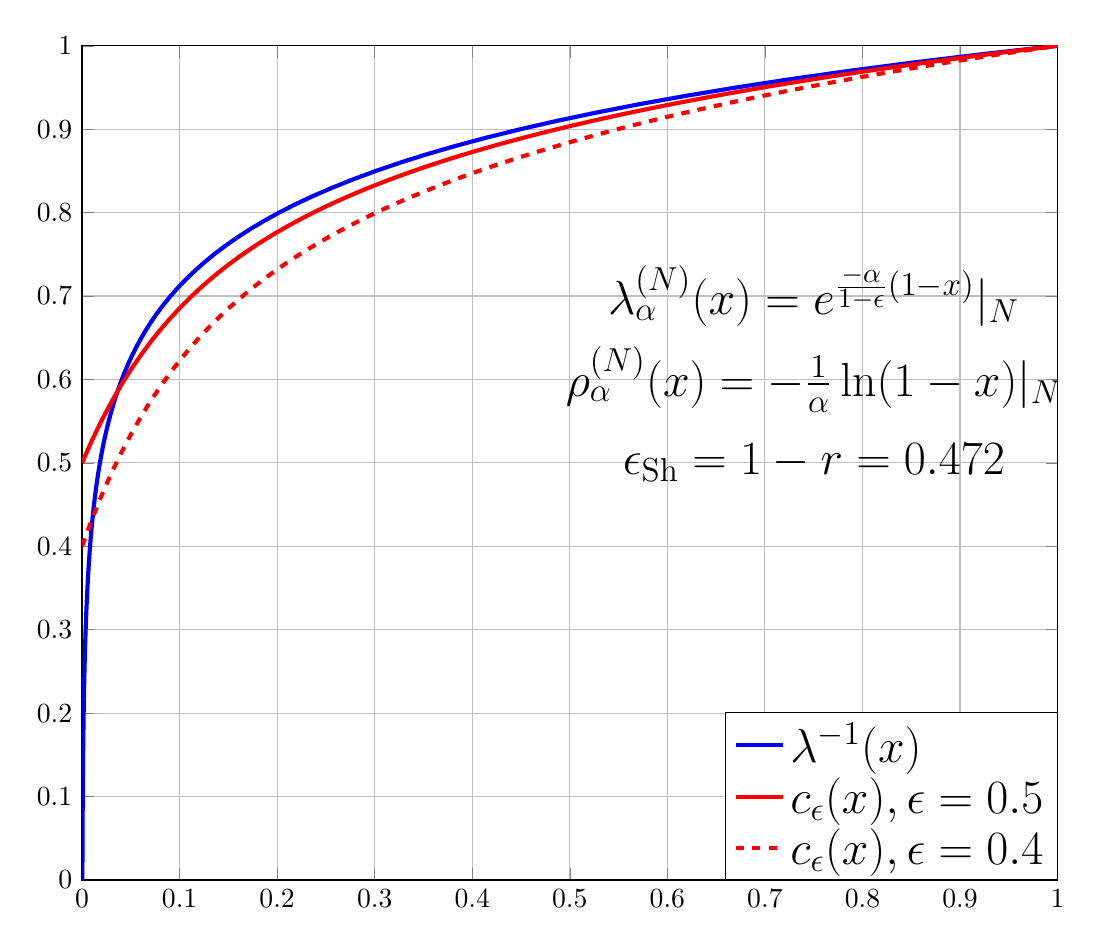
\begin{tikzpicture}
\def\fsize{\LARGE}

\begin{axis}[%
width=4.87804024496938in,
height=4.17068372703412in,
scale only axis,
xmin=0,
xmax=1,
xmajorgrids,
xtick={0,0.1,0.2,...,1},
xticklabels={0,0.1,0.2,0.3,0.4,0.5,0.6,0.7,0.8,0.9,1},
ymin=0,
ymax=1,
legend style={at={(1,0)},anchor=south east,draw=black,fill=white,legend cell align=left,font=\LARGE},
ymajorgrids
]
\node at (axis cs:0.75,0.7){\fsize{$\lambda_{\alpha}^{(N)}(x)=e^{\frac{-\alpha}{1-\epsilon} (1-x)}|_{N}$}};
%\sum\limits_{i=1}^{N}\frac{1}{\alpha}\frac{x^i}{i}}};
\node at (axis cs:0.75,0.6){\fsize{$\rho_{\alpha}^{(N)}(x)=-\frac{1}{\alpha}\ln (1-x)|_{N}$}};
%x^{\frac{1}{\alpha}},\alpha=0.1,N=50$}};
\node at (axis cs:0.75,0.5){\fsize{$\epsilon_{\text{Sh}}=1-r=0.472$}};

\addlegendentry{$\lambda^{-1}(x)$};
\addplot [color=blue,solid,line width=1.5pt]
  table[row sep=crcr]{0.000335494153584825	0\\
0.000363436477858997	0.01\\
0.000393706036385988	0.02\\
0.000426496657682508	0.03\\
0.000462018313674054	0.04\\
0.000500498464232096	0.05\\
0.000542183513693807	0.06\\
0.00058734038869107	0.07\\
0.000636258247392219	0.08\\
0.000689250331101526	0.09\\
0.000746655970072966	0.1\\
0.000808842756382345	0.11\\
0.000876208897771561	0.12\\
0.000949185767537662	0.13\\
0.00102824066679468	0.14\\
0.00111387981679615	0.15\\
0.00120665160047942	0.16\\
0.00130715007398865	0.17\\
0.00141601877066227	0.18\\
0.00153395482184343	0.19\\
0.00166171342090063	0.2\\
0.00180011265904357	0.21\\
0.00195003876389988	0.22\\
0.0021124517743976	0.23\\
0.00228839168829194	0.24\\
0.00247898512170151	0.25\\
0.00268545252329786	0.26\\
0.00290911598934362	0.27\\
0.00315140772962231	0.28\\
0.00341387923847058	0.29\\
0.00369821122963888	0.3\\
0.00400622439859745	0.31\\
0.00433989108120327	0.32\\
0.00470134788338308	0.33\\
0.00509290936270569	0.34\\
0.00551708284945217	0.35\\
0.00597658450208934	0.36\\
0.00647435669995645	0.37\\
0.00701358688453719	0.38\\
0.00759772796996556	0.39\\
0.00823052045346203	0.4\\
0.00891601636728181	0.41\\
0.00965860522554881	0.42\\
0.0104630421321226	0.43\\
0.0113344782294832	0.44\\
0.0122784936836085	0.45\\
0.0133011334160577	0.46\\
0.0144089458120634	0.47\\
0.0156090246524914	0.48\\
0.0169090545381691	0.49\\
0.0183173600974417	0.5\\
0.0198429592920402	0.51\\
0.0214956211625829	0.52\\
0.0232859283834527	0.53\\
0.0252253450275842	0.54\\
0.0273262899750436	0.55\\
0.0296022164354101	0.56\\
0.0320676980931018	0.57\\
0.0347385224271733	0.58\\
0.0376317918030286	0.59\\
0.0407660329832215	0.6\\
0.0441613157583836	0.61\\
0.0478393814576613	0.62\\
0.0518237821612379	0.63\\
0.0561400315059548	0.64\\
0.060815768049174	0.65\\
0.0658809322363014	0.66\\
0.0713679581043317	0.67\\
0.0773119809479292	0.68\\
0.0837510622765184	0.69\\
0.0907264335012647	0.7\\
0.098282759910384	0.71\\
0.106468426620664	0.72\\
0.115335848333247	0.73\\
0.124941804873458	0.74\\
0.135347804658769	0.75\\
0.146620478416798	0.76\\
0.15883200566779	0.77\\
0.172060576694392	0.78\\
0.186390892947055	0.79\\
0.201914709077521	0.8\\
0.218731420056951	0.81\\
0.23694869712112	0.82\\
0.256683176594334	0.83\\
0.278061205978336	0.84\\
0.301219652054399	0.85\\
0.326306776138336	0.86\\
0.353483182051611	0.87\\
0.382922842829663	0.88\\
0.41481421268376	0.89\\
0.449361431268097	0.9\\
0.486785627882633	0.91\\
0.527326333867846	0.92\\
0.571243012123746	0.93\\
0.618816713416241	0.94\\
0.670351869923472	0.95\\
0.726178237327734	0.96\\
0.786652997679963	0.97\\
0.852163036258837	0.98\\
0.923127406721123	0.99\\
1	1\\
};

\addlegendentry{$c_{\epsilon}(x),\epsilon=0.5$};
\addplot [color=red,solid,line width=1.5pt]
  table[row sep=crcr]{0	0.5\\
0.01	0.526526126042806\\
0.02	0.550706243040251\\
0.03	0.57280262188789\\
0.04	0.593046195873519\\
0.05	0.6116403489369\\
0.06	0.628764252863599\\
0.07	0.644575805441883\\
0.08	0.659214215869252\\
0.09	0.672802278552915\\
0.1	0.685448371847462\\
0.11	0.697248214159826\\
0.12	0.708286406177705\\
0.13	0.718637784699063\\
0.14	0.728368610616949\\
0.15	0.73753761100972\\
0.16	0.746196892968877\\
0.17	0.754392744735548\\
0.18	0.762166337885451\\
0.19	0.769554342676617\\
0.2	0.776589467232609\\
0.21	0.783300929956643\\
0.22	0.789714873441285\\
0.23	0.795854727138328\\
0.24	0.801741525169708\\
0.25	0.807394184880162\\
0.26	0.812829751044085\\
0.27	0.818063610032608\\
0.28	0.82310967771285\\
0.29	0.827980564381521\\
0.3	0.832687719622072\\
0.31	0.837241559611941\\
0.32	0.841651579088144\\
0.33	0.84592644990045\\
0.34	0.850074107836845\\
0.35	0.854101829192009\\
0.36	0.858016298362217\\
0.37	0.861823667586471\\
0.38	0.865529609810601\\
0.39	0.869139365526266\\
0.4	0.87265778432787\\
0.41	0.876089361835362\\
0.42	0.879438272548156\\
0.43	0.882708399123219\\
0.44	0.885903358507587\\
0.45	0.889026525300862\\
0.46	0.892081052675632\\
0.47	0.89506989114236\\
0.48	0.897995805409208\\
0.49	0.900861389555933\\
0.5	0.903669080713676\\
0.51	0.906421171418762\\
0.52	0.909119820787906\\
0.53	0.911767064644275\\
0.54	0.914364824708154\\
0.55	0.91691491695232\\
0.56	0.919419059210307\\
0.57	0.921878878115366\\
0.58	0.924295915438839\\
0.59	0.926671633888754\\
0.6	0.929007422422485\\
0.61	0.931304601121274\\
0.62	0.93356442566907\\
0.63	0.935788091473473\\
0.64	0.937976737462459\\
0.65	0.94013144958696\\
0.66	0.94225326405617\\
0.67	0.944343170329661\\
0.68	0.946402113887892\\
0.69	0.948430998800506\\
0.7	0.950430690109856\\
0.71	0.952402016045493\\
0.72	0.954345770083781\\
0.73	0.95626271286546\\
0.74	0.958153573982763\\
0.75	0.960019053646566\\
0.76	0.961859824243142\\
0.77	0.963676531789142\\
0.78	0.965469797292704\\
0.79	0.967240218027864\\
0.8	0.968988368728802\\
0.81	0.970714802709912\\
0.82	0.972420052917143\\
0.83	0.974104632915626\\
0.84	0.97576903781815\\
0.85	0.977413745158703\\
0.86	0.979039215714913\\
0.87	0.980645894282958\\
0.88	0.982234210408185\\
0.89	0.983804579074453\\
0.9	0.985357401354956\\
0.91	0.986893065027096\\
0.92	0.988411945153746\\
0.93	0.989914404633095\\
0.94	0.991400794719091\\
0.95	0.992871455514339\\
0.96	0.994326716437194\\
0.97	0.995766896664656\\
0.98	0.997192305552543\\
0.99	0.998603243034339\\
1	1\\
};

\addlegendentry{$c_{\epsilon}(x),\epsilon=0.4$};
\addplot [color=red,dashed,line width=1.5pt]
  table[row sep=crcr]{0	0.4\\
0.01	0.431831351251367\\
0.02	0.460847491648301\\
0.03	0.487363146265468\\
0.04	0.511655435048223\\
0.05	0.533968418724279\\
0.06	0.554517103436319\\
0.07	0.57349096653026\\
0.08	0.591057059043103\\
0.09	0.607362734263498\\
0.1	0.622538046216955\\
0.11	0.63669785699179\\
0.12	0.649943687413245\\
0.13	0.662365341638875\\
0.14	0.674042332740338\\
0.15	0.685045133211665\\
0.16	0.695436271562653\\
0.17	0.705271293682658\\
0.18	0.714599605462541\\
0.19	0.723465211211941\\
0.2	0.731907360679131\\
0.21	0.739961115947971\\
0.22	0.747657848129542\\
0.23	0.755025672565993\\
0.24	0.76208983020365\\
0.25	0.768873021856194\\
0.26	0.775395701252902\\
0.27	0.781676332039129\\
0.28	0.78773161325542\\
0.29	0.793576677257825\\
0.3	0.799225263546487\\
0.31	0.804689871534329\\
0.32	0.809981894905773\\
0.33	0.81511173988054\\
0.34	0.820088929404215\\
0.35	0.82492219503041\\
0.36	0.82961955803466\\
0.37	0.834188401103766\\
0.38	0.838635531772721\\
0.39	0.84296723863152\\
0.4	0.847189341193444\\
0.41	0.851307234202435\\
0.42	0.855325927057787\\
0.43	0.859250078947862\\
0.44	0.863084030209105\\
0.45	0.866831830361034\\
0.46	0.870497263210758\\
0.47	0.874083869370832\\
0.48	0.87759496649105\\
0.49	0.881033667467119\\
0.5	0.884402896856411\\
0.51	0.887705405702515\\
0.52	0.890943784945487\\
0.53	0.89412047757313\\
0.54	0.897237789649784\\
0.55	0.900297900342784\\
0.56	0.903302871052369\\
0.57	0.906254653738439\\
0.58	0.909155098526607\\
0.59	0.912005960666505\\
0.6	0.914808906906982\\
0.61	0.917565521345529\\
0.62	0.920277310802884\\
0.63	0.922945709768168\\
0.64	0.925572084954951\\
0.65	0.928157739504352\\
0.66	0.930703916867404\\
0.67	0.933211804395593\\
0.68	0.935682536665471\\
0.69	0.938117198560607\\
0.7	0.940516828131827\\
0.71	0.942882419254591\\
0.72	0.945214924100537\\
0.73	0.947515255438552\\
0.74	0.949784288779315\\
0.75	0.952022864375879\\
0.76	0.954231789091771\\
0.77	0.95641183814697\\
0.78	0.958563756751245\\
0.79	0.960688261633437\\
0.8	0.962786042474563\\
0.81	0.964857763251894\\
0.82	0.966904063500572\\
0.83	0.968925559498751\\
0.84	0.970922845381781\\
0.85	0.972896494190444\\
0.86	0.974847058857895\\
0.87	0.976775073139549\\
0.88	0.978681052489822\\
0.89	0.980565494889343\\
0.9	0.982428881625947\\
0.91	0.984271678032515\\
0.92	0.986094334184495\\
0.93	0.987897285559714\\
0.94	0.98968095366291\\
0.95	0.991445746617207\\
0.96	0.993192059724633\\
0.97	0.994920275997587\\
0.98	0.996630766663051\\
0.99	0.998323891641207\\
1	1\\
};
\end{axis}
\end{tikzpicture}}
\end{center}
\column{0.45\textwidth}
\begin{center}
  \includegraphics[width=2.2in]{./Figures/ratelesserasures3}
\end{center}
\end{columns}
%\begin{block}{Poisson, Soliton pair is optimal - $\lambda(x) = e^{-r_{avg}(1-x)}$}
\begin{itemize}
%\item Poisson, soliton pair is optimal 
  %\item Left degree is Poisson : $\lambda(x) = e^{-r_{avg}(1-x)}$
  \item   $x = \lambda(1-(1-\epsilon)\rho(1-x))$
  \item $\lambda(x) = e^{-\frac{\alpha}{1-\epsilon}(1-x)}$, \alert{Optimal right degree is soliton: $\rho(x) = -\frac{1}{\alpha}\ln(1-x)$}
  %\item \alert{Optimal distribution is soliton: $f_D[i] = \frac{1}{i(i-1)}$}
\end{itemize}
\begin{center}
\begin{tabular}{|l|c|c|c|c|c|c|}
\hline
Degree of nodes & 1 & 2 & 3 & 4 & $\ldots$ & $K$ \\
\hline
Fraction: \alert{ $f_D[i] = \frac{1}{i(i-1)}$ } & 0 & $\frac12$ & $\frac16$ & $\frac{1}{12}$ & $\ldots$ & $\frac{1}{K (K-1)}$ \\
\hline
\end{tabular}
\end{center}
%\end{block}
\end{frame}
%--------------------------------------------------------------------------------------
\begin{frame}{Histogram of required $N$ for $K=10000$}
\begin{center}
  \includegraphics[width=4.2in]{./Figures/fountaincodes10000histogram}
\end{center}
\begin{block}{Finite length considerations}
\begin{itemize}
  \item Deg. dist. must be adjusted for optimizing finite length performance
  \item Raptor codes (Shokrollahi'06) is an excellent choice
\end{itemize}
\end{block}
\end{frame}
%--------------------------------------------------------------------------------------
\begin{frame}\frametitle{Erasures to errors - Tensoring and Peeling}
\begin{columns}
    \column{.45\textwidth}
    \small
    \[
    H = \left[
    \begin{array}{ccccccc}
    1&0&1&1&0&0\\
    1&1&0&0&1&0 \\
    0&1&1&0&0&1
    \end{array}
    \right]
    \]
    \[
    \otimes
    \]
    \[
    T = \left[
    \begin{array}{ccccccc}
    1&1&1&1&1&1\\
    1&W&W^2&W^3&W^4&W^5
    \end{array}
    \right]
    \]
    \[
    \mathbf{\tilde{H}} = \left[
    \begin{array}{ccccccc}
    1&0&1&1&0&0\\
    1&0&W^2&W^3&0&0\\
    1&1&0&0&1&0 \\
    1&W&0&0&W^4&0 \\
    0&1&1&0&0&1 \\
    0&W&W^2&0&0&W^5
    \end{array}
    \right]
    \]
    \column{.45\textwidth}
    \begin{figure}[t]
    \centering
    \includegraphics[width=2.0in,angle=-90]{./Figures/GLDPC}
    \end{figure}
\end{columns}

\begin{itemize}
\item $W$ is a primitive element in the field
\item Each check is a 1-error correcting code
\item If there is exactly one error in a check, it can be recovered
\end{itemize}

\end{frame}
%--------------------------------------------------------------------------------------
\begin{frame}{Peeling process is same for erasure and error channels}
\begin{columns}
\column{0.5\textwidth}
\includegraphics[width=2.3in,angle=-90]{./Figures/Tannergraph63codewitherasures}
\column{0.5\textwidth}
\includegraphics[width=2.25in,angle=-90]{./Figures/GLDPC}
\end{columns}
\begin{block}{}
\begin{itemize}
  \item Assume no miscorrection by the check code
  \item One-to-one correspondence between messages passed - DE can be used
  \item Not optimal for the error channel but it is not bad at high rates
\end{itemize}
\end{block}
\end{frame}
%--------------------------------------------------------------------------------------
\begin{frame}{Generalized LDPC Code}

\begin{columns}
    \column{.6\textwidth}
    .
%    \small
%    \[
%    H = \left[
%    \begin{array}{ccccccc}
%    1&0&1&1&0&0\\
%    1&1&0&0&1&0 \\
%    0&1&1&0&0&1
%    \end{array}
%    \right]
%    \]
%    \[
%    \otimes
%    \]
%    \[
%    T = \left[
%    \begin{array}{ccccccc}
%    1&1&1&1&1&1\\
%    1&W&W^2&W^3&W^4&W^5 \\
%    \vdots & \vdots & \vdots & \vdots & \vdots & \vdots \\
%    1&W^{2t-1}&W^{2(2t-1)}&\cdots&\cdots&W^{5(2t-1)}
%    \end{array}
%    \right]
%    \]
%    \[
%    \mathbf{\tilde{H}} = H \otimes T
%    \]
    \column{.4\textwidth}
    \begin{figure}[t]
    \centering
    \includegraphics[width=2.0in,angle=-90]{./Figures/GLDPC}
    \end{figure}
\end{columns}

\begin{itemize}
\item GLDPC introduced by Tanner in 1981
\item Each check is a $t$-error correcting code
\item If there are exactly $t$ errors in a check, it can be recovered
\item Density evolution equations can be written and thresholds computed
\end{itemize}

\end{frame}
%--------------------------------------------------------------------------------------
\begin{frame}{Generalized LDPC Code}

\begin{columns}
    \column{.6\textwidth}
    \small
    \[
    H = \left[
    \begin{array}{ccccccc}
    1&0&1&1&0&0\\
    1&1&0&0&1&0 \\
    0&1&1&0&0&1
    \end{array}
    \right]
    \]
    \[
    \otimes
    \]
    \[
    T = \left[
    \begin{array}{ccccccc}
    1&1&1&1&1&1\\
    1&W&W^2&W^3&W^4&W^5 \\
    \vdots & \vdots & \vdots & \vdots & \vdots & \vdots \\
    1&W^{2t-1}&W^{2(2t-1)}&\cdots&\cdots&W^{5(2t-1)}     
    \end{array}
    \right]
    \]
    \[
    \mathbf{\tilde{H}} = H \otimes T
    \]
    \column{.4\textwidth}
    \begin{figure}[t]
    \centering
    \includegraphics[width=2.0in,angle=-90]{./Figures/GLDPC}
    \end{figure}
\end{columns}

\begin{itemize}
\item $W$ is a primitive element in the field
\item Each check is a $t$-error correcting RS code
\item If there are exactly $t$ errors in a check, it can be recovered
\end{itemize}

\end{frame}
%--------------------------------------------------------------------------------------
\begin{frame}{Product Code}
\begin{itemize}
\item Special case of generalized LDPC code
\item Let component code $\mathcal{C}$ be an $(n,k,d_{\text{min}})$ linear code
\item Well-known that \textcolor{blue}{$\mathcal{P}$ is an $(n^{2},k^{2},d_{\text{min}}^{2})$
linear code }
\end{itemize}

\begin{center}
\scalebox{0.8}{\tikzset
{
    vnodeStyle/.style =
    {
        % -- shape properties --
        circle,                                 % shape
        minimum size    = 7mm,                %
        scale           = 1.0,                  % scaling factor
        thick,                                  % thickness of the border
        %
        % -- colours properties --
        % filling: [ trasparent | monocolored | shaded]; decomment what you prefer
%       %                                       % transparent (all commented)
        fill            = yellow!10,             % monocolored
        text            = black,                % colour of the fonts
        draw            = black,                % colour of the border
        %
        % -- fonts --
        font            = \scriptsize,              % shape of the font (or dimension, like \tiny)
%       text centered,                          % text alignment [text centered | text badly centered | text justified | text ragged | text badly ragged]
        inner xsep      = 0mm,                  % minimum distance between text and borders along x dimension
        inner ysep      = 0mm,                  % minimum distance between text and borders along y dimension
        text height     = 0.2cm,
        text depth      = 0.12cm,
    }
}

%\begin{center}
\tikzstyle{styB}=[circle,
  ball color=blue,
  inner sep=0pt,
  minimum size=10pt]
\tikzstyle{styKB}=[circle,
  ball color=blue!10!white,
  inner sep=0pt,
  minimum size=10pt]
\tikzstyle{styCd}=[rectangle, draw=blue!50,
  top color=blue!40!white, bottom color=blue!10,
  inner sep=0pt,
  minimum size=10pt]
\tikzstyle{styCu}=[rectangle, draw=blue,
  top color=blue, bottom color=blue!40,
  inner sep=0pt,
  minimum size=10pt]

\pgfdeclarelayer{background}
%
\pgfdeclarelayer{foreground}
%
\pgfdeclarelayer{m-f}
%
\pgfdeclarelayer{main}
%
\pgfsetlayers{background,main,m-f,foreground}

\begin{tikzpicture}[scale=2.0]
% \draw[step=5mm,color=gray!40!white, thin] (0,0) grid (12,5);

\colorlet{uecolr}{black} \colorlet{decolr}{black!40}

\def\strt  {-40mm}
\def\shf   {10mm}
\def\ang   {55}
\def\dist  {4mm}
\def\cvd   {18mm}

\def\n     {6}
\def\s     {7}

\begin{scope}[xshift=-7cm, yshift=-1.2cm]

\only<1>
{
%\node (cc) at (12mm,5mm) {Product Code\vphantom{y}};

\foreach \rr in {0,1,...,\n}
 \foreach \cc in {0,1,...,\n}
  \node[vnodeStyle] (p\rr\cc) at (\rr*4mm,-\cc*4mm) {$X_{\cc,\rr}$};

 \node [rectangle,rounded corners=2mm,minimum width=7mm,minimum height=55mm,draw=red,thick] (circ1) at (4mm,-12mm) {};
 \node [rectangle,rounded corners=2mm,minimum width=55mm,minimum height=7mm,draw=red,thick] (circ2) at (12mm,-4mm) {};
}

\only<2>
{
%\node (cc) at (12mm,5mm) {Product Code\vphantom{y}};

\foreach \rr in {0,1,...,\n}
 \foreach \cc in {0,1,...,\n}
  \node[vnodeStyle] (p\rr\cc) at (\rr*4mm,-\cc*4mm) {$X_{\cc,\rr}$};

 \node [rectangle,rounded corners=2mm,minimum width=39mm,minimum height=39mm,draw=black,thick] (circ1) at (8mm,-8mm) {};
 \node [rectangle,rounded corners=2mm,minimum width=14mm,minimum height=55mm,draw=blue,thick] (circ1) at (22mm,-12mm) {};
 \node [rectangle,rounded corners=2mm,minimum width=55mm,minimum height=14mm,draw=red,thick] (circ2) at (12mm,-22mm) {};
}

%\only<2>
%{
%\node (cc) at (12mm,5mm) {Symmetric Subcode};
%
%\foreach \cc in {0,1,...,\n}
%  \foreach \rr in {\cc,...,\n}
%    \node[vnodeStyle] (p\rr\cc) at (\rr*4mm,-\cc*4mm) {$X_{\cc,\rr}$};
%
%\pgfmathtruncatemacro{\nnn}{\n-1}
%\foreach \rr in {0,1,...,\nnn} {
%  \pgfmathtruncatemacro{\rrr}{\rr+1}
%  \foreach \cc in {\rrr,...,\n}
%    \node[vnodeStyle] (p\rr\cc) at (\rr*4mm,-\cc*4mm) {$X_{\color{red}{\rr,\cc}}$};
%}
%
% \node [rectangle,rounded corners=2mm,minimum width=7mm,minimum height=55mm,draw=red,thick] (circ1) at (4mm,-12mm) {};
% \node [rectangle,rounded corners=2mm,minimum width=55mm,minimum height=7mm,draw=red,thick] (circ2) at (12mm,-4mm) {};
%}

%\only<3>
%{
%\node (cc) at (12mm,5mm) {Punctured Symmetric Subcode};
%
%\foreach \cc in {0,1,...,\n}
%  \foreach \rr in {\cc,...,\n}
%    \node[vnodeStyle] (p\rr\cc) at (\rr*4mm,-\cc*4mm) {$X_{\cc,\rr}$};
%
% \node [rectangle,rounded corners=2mm,minimum width=7mm,minimum height=15mm,draw=red,thick] (circ1) at (4mm,-2mm) {};
% \node [rectangle,rounded corners=2mm,minimum width=47mm,minimum height=7mm,draw=red,thick] (circ2) at (14mm,-4mm) {};
%}


%\foreach \rr in {0,1,...,\n}{
% \node [rectangle,rounded corners=1mm,minimum width=4mm,minimum height=\n*4mm+4mm,draw=red,thick] (circ1) at (1*4mm,3*4mm) {};
% \node [rectangle,rounded corners=1mm,minimum width=\n*4mm+4mm,minimum height=4mm,draw=maroon,thick] (circ2) at (3*4mm,1*4mm) {};
% \node (cc) at (12mm,29mm) {column codewords};
% \node [rotate=90](rc) at (-6mm,12mm) {row codewords};
% }
\end{scope}

\end{tikzpicture}
%\end{center}
}
\end{center}
\end{frame}

%--------------------------------------------------------------------------------------
\begin{frame}{\alert{Peeling} decoding of Product Codes}

\begin{itemize}
\item \textcolor{blue}{Hard-decision ``cascade decoding''} by Abramson in 1968
\item Identical to a \alert{peeling decoder}
\item Example: $t=2$-error-correcting codes, bounded distance decoding
\end{itemize}

\begin{columns}
\begin{column}{0.5\textwidth}
\scalebox{1.4}{\pgfdeclarelayer{background}
\pgfdeclarelayer{foreground}
\pgfdeclarelayer{m-f}
\pgfdeclarelayer{main}

\pgfsetlayers{background,foreground}

\begin{tikzpicture}[scale=1.0]
\clip  (-2mm,-2mm) rectangle (26mm, 26mm); 

\def\n     {6}

\begin{pgfonlayer}{background}
%\draw[gray,step=2mm] (-2mm,-2mm) grid (26mm, 26mm);
\foreach \rr in {0,1,...,\n}
 \foreach \cc in {0,1,...,\n}{
  \node[vnodeStyle] (p\rr\cc) at (\rr*4mm,\cc*4mm) {};
 }
\end{pgfonlayer}

\begin{pgfonlayer}{foreground}
\uncover<2-2>{
 \node[minimum width=10cm] (txt) at (12mm,-8mm) {Received block};
}

\uncover<2-3>{
 \foreach \rr/\cc in {1/0,2/0,2/1,0/5,1/4,0/4,6/3,2/4,6/4,3/2,1/3,4/5,3/6,2/2,6/6,6/1}{
  \node[vnodeStyle,thick,fill=red!50,draw=red!80!black!80] (it1\rr\cc)
  at (\cc*4mm,\rr*4mm) {};
 }
}

\uncover<3-4>{
 \node[minimum width=10cm] (txt) at (12mm,-8mm) {Row decoding};
}

\uncover<3-3>{
 \node [rectangle,rounded corners=1mm,minimum width=\n*4mm+4mm,minimum height=4mm,draw=blue,thick] (circ2) at (3*4mm,4*4mm) {};
 \node [rectangle,rounded corners=1mm,minimum width=\n*4mm+4mm,minimum height=4mm,draw=blue,thick] (circ2) at (3*4mm,3*4mm) {};
 \node [rectangle,rounded corners=1mm,minimum width=\n*4mm+4mm,minimum height=4mm,draw=blue,thick] (circ2) at (3*4mm,0*4mm) {};
}

\uncover<4-6>{
 \foreach \rr/\cc in {1/0,2/0,2/1,1/4,6/3,2/4,6/4,1/3,2/2,6/6,6/1}{
  \node[vnodeStyle,thick,fill=red!50,draw=red!80!black!80] (it1\rr\cc)
  at (\cc*4mm,\rr*4mm) {};
 }
}

\uncover<5-6>{
 \node[minimum width=10cm] (txt) at (12mm,-8mm) {Column decoding};
}

\uncover<6-6>{
 \node [rectangle,rounded corners=1mm,minimum width=4mm,minimum height=\n*4mm+4mm,draw=blue,thick] (circ1) at (0*4mm,3*4mm) {};
 \node [rectangle,rounded corners=1mm,minimum width=4mm,minimum height=\n*4mm+4mm,draw=blue,thick] (circ1) at (1*4mm,3*4mm) {};
 \node [rectangle,rounded corners=1mm,minimum width=4mm,minimum height=\n*4mm+4mm,draw=blue,thick] (circ1) at (2*4mm,3*4mm) {};
 \node [rectangle,rounded corners=1mm,minimum width=4mm,minimum height=\n*4mm+4mm,draw=blue,thick] (circ1) at (3*4mm,3*4mm) {};
 \node [rectangle,rounded corners=1mm,minimum width=4mm,minimum height=\n*4mm+4mm,draw=blue,thick] (circ1) at (5*4mm,3*4mm) {};
 \node [rectangle,rounded corners=1mm,minimum width=4mm,minimum height=\n*4mm+4mm,draw=blue,thick] (circ1) at (6*4mm,3*4mm) {};
}

\uncover<7-7>{
 \foreach \rr/\cc in {1/4,2/4,6/4}{
  \node[vnodeStyle,thick,fill=red!50,draw=red!80!black!80] (it1\rr\cc)
  at (\cc*4mm,\rr*4mm) {};
 }
}

\uncover<8-8>{
 \node[minimum width=10cm] (txt) at (12mm,-8mm) {Decoding successful};
}


\uncover<9-9>{
 \node[minimum width=10cm] (txt) at (12mm,-8mm) {Or trapped in a \textcolor{red}{stopping set}};
 \foreach \rr/\cc in {1/0,3/0,6/0,1/2,3/2,6/2,1/5,3/5,6/5}{
  \node[vnodeStyle,thick,fill=red!50,draw=red!80!black!80] (it1\rr\cc)
  at (\cc*4mm,\rr*4mm) {};
 }
}
\end{pgfonlayer}
\end{tikzpicture}}
\end{column}

\begin{column}{0.5\textwidth}
\begin{figure}[t]
\centering
\includegraphics[width=1.5in]{./Figures/Bipartite_graph}
\end{figure}
\end{column}
\end{columns}
\end{frame}
%---------------------------------------------------------------------------------------
	\begin{frame}{Density Evolution(DE) for Product Codes -Justesen et al}
	%   Slide-1:
	%   \begin{itemize}
	%   	\item Introduce the main idea of Justesen's analysis (establish the assumptions in the beginning)
	%   \end{itemize}
	%   Slide-2:
	%   \begin{itemize}
	%   	\item Tail of the Poisson Distribution. Notion of $\pi_{t}(m)$.
	%   	\item Effect- of first step of decoding. Equation for the new mean in therms of $\pi_t(M)$.
	%   \end{itemize}
	
	   \begin{columns}
	   	\column{0.72\textwidth}
	   	
	   	\begin{block}{Assumptions}
	   		
	   		\begin{itemize}
	   			\item $P_1=P_2 = P$
	   			\item Errors are \alert{randomly distributed} in rows and columns
	   			\item If $P \gg t$, \alert{\# errors} in each row/col $\sim$ \alert{Poisson}($M$))
	   		\end{itemize}
	   	\end{block}
	   	\pause
	   	\begin{block}{Main Idea}
	   		\begin{itemize}
	   			%\item Random \alert{bipartite graph} - row and column codes
	   			\item Removal of \alert{corrected vertices} (degree$\leq t$) from row codes $\Leftrightarrow$ removal of random edges from column codes
	   			\item \# of errors in row/column changes after each iter
	   			\begin{itemize}
	   				\item Track the distribution
	   				%\item Changes the Poisson parameter ($m(j)$)
	   				%\item \alert{Threshold} - max. $M$ such that $m(j) \rightarrow 0$ as $j \rightarrow \infty$
	   			\end{itemize}
	   			%\item Generalize for $d \geq 2$
	   		\end{itemize}
	   	\end{block}
	   	\column{0.25\textwidth}
	   	 	
	   	\begin{figure}[t]
	   		\centering
	   		\includegraphics[width=1.3in]{./Figures/Bipartite_graph}
	   	\end{figure}
	   		
	   \end{columns}
	
	\end{frame}
	%--------------------------------------------------------------------------------------
	\begin{frame}{DE continued}
		\begin{block}{Tail of the Poisson distribution}
			\begin{equation}\nonumber
			\pi_t(m) = \sum_{j \geq t} \mathrm{e}^{-m}m^j/j!
			\label{eqn:defpi}
			\end{equation}
		\end{block}
		
		\begin{block}{Effect of first step of decoding}
			If the \# errors is poisson with mean $M$, Mean \# of errors after decoding is
			\begin{equation}\nonumber
			\textcolor{blue}{m(1)} = \sum_{j \geq t+1} j\mathrm{e}^{-M}M^j/j! = M\pi_t(M)
			\label{eqn:defpi}
			\end{equation}
		\end{block}
		
	\end{frame}
	%----------------------------------------------------------------------------------------
	\begin{frame}{Evolution of degree distribution($d=2$) - first iteration}
	
	%	Slide-1: First iteration
	%	\begin{itemize}
	%		\item Figures: Graphs showing how the distribution changes before/after row/column decoding in the first iteration
	%	\end{itemize}
	%	Slide-2: jth iteration
	%	\begin{itemize}
	%		\item Figures: Degree distribution for jth iteration.
	%		\item Equations showing the relation between two successive means.
	%	\end{itemize}
	
		\begin{columns}
			
			\column{0.5\textwidth}
			{\vspace{-6mm}
				\hspace{6mm}
				\begin{block}{Before row decoding}
					{\color{blue}Distribution}: Poisson($M$) \\
					{\color{blue}Mean}: $M$
				\end{block}}
				
				\begin{block}{After row decoding}
					{\color{blue}Distribution}: Truncated Poisson($M$) \\
					{\color{blue}Mean}: $M \pi_t(M) = m(1)$
				\end{block}
				
				\begin{block}{Before column decoding}
					{\color{blue}Distribution}: Poisson($m(1)$) \\
					{\color{blue}Mean}: $m(1)$
				\end{block}
				
				\begin{block}{After column decoding}
					{\color{blue}Distribution}: Truncated Poisson($m(1)$) \\
					%{\color{blue}Mean}: $m(2) = M \pi_t(m(1))$
				\end{block}
				
				
				\column{0.5\textwidth}
				\begin{center}
					\vspace{-3mm}
					% This file was created by matlab2tikz.
%
%The latest updates can be retrieved from
%  http://www.mathworks.com/matlabcentral/fileexchange/22022-matlab2tikz-matlab2tikz
%where you can also make suggestions and rate matlab2tikz.
%
\definecolor{mycolor1}{rgb}{0.00000,0.44700,0.74100}%
%
\begin{tikzpicture}

\begin{axis}[%
width=1.521in,
height=0.566in,
at={(0.758in,0.481in)},
scale only axis,
xmin=0,
xmax=15,
ymin=0,
ymax=0.25,
axis background/.style={fill=white}
]
\addplot[ycomb,color=mycolor1,solid,mark=o,mark options={solid},forget plot] plot table[row sep=crcr] {%
0	0.0497870683678639\\
1	0.149361205103592\\
2	0.224041807655388\\
3	0.224041807655388\\
4	0.168031355741541\\
5	0.100818813444924\\
6	0.0504094067224623\\
7	0.0216040314524838\\
8	0.00810151179468143\\
9	0.00270050393156048\\
10	0.000810151179468142\\
11	0.00022095032167313\\
12	5.52375804182826e-05\\
13	1.27471339426806e-05\\
14	2.73152870200298e-06\\
15	5.46305740400597e-07\\
};
\end{axis}
\end{tikzpicture}%
					% This file was created by matlab2tikz.
%
%The latest updates can be retrieved from
%  http://www.mathworks.com/matlabcentral/fileexchange/22022-matlab2tikz-matlab2tikz
%where you can also make suggestions and rate matlab2tikz.
%
\definecolor{mycolor1}{rgb}{0.00000,0.44700,0.74100}%
%
\begin{tikzpicture}

\begin{axis}[%
width=1.521in,
height=0.566in,
at={(0.758in,0.481in)},
scale only axis,
xmin=0,
xmax=15,
ymin=0,
ymax=0.3,
axis background/.style={fill=white}
]
\addplot[ycomb,color=mycolor1,solid,mark=o,mark options={solid},forget plot] plot table[row sep=crcr] {%
0	0\\
1	0\\
2	0.279754460090289\\
3	0.279754460090289\\
4	0.209815845067717\\
5	0.12588950704063\\
6	0.0629447535203151\\
7	0.0269763229372779\\
8	0.0101161211014792\\
9	0.00337204036715975\\
10	0.00101161211014792\\
11	0.000275894211858524\\
12	6.89735529646311e-05\\
13	1.59169737610687e-05\\
14	3.41078009165758e-06\\
15	6.82156018331516e-07\\
};
\end{axis}
\end{tikzpicture}%
					% This file was created by matlab2tikz.
%
%The latest updates can be retrieved from
%  http://www.mathworks.com/matlabcentral/fileexchange/22022-matlab2tikz-matlab2tikz
%where you can also make suggestions and rate matlab2tikz.
%
\definecolor{mycolor1}{rgb}{0.00000,0.44700,0.74100}%
%
\begin{tikzpicture}

\begin{axis}[%
width=1.521in,
height=0.566in,
at={(0.758in,0.481in)},
scale only axis,
xmin=0,
xmax=15,
ymin=0,
ymax=0.4,
axis background/.style={fill=white}
]
\addplot[ycomb,color=mycolor1,solid,mark=o,mark options={solid},forget plot] plot table[row sep=crcr] {%
0	0.347043782149382\\
1	0.367277938616125\\
2	0.194345917046349\\
3	0.0685590420793257\\
4	0.0181390828359174\\
5	0.00383933399474955\\
6	0.000677197300830985\\
7	0.000102382976886822\\
8	1.35440435164562e-05\\
9	1.59263554985051e-06\\
10	1.68549310433711e-07\\
11	1.62160423332975e-08\\
12	1.43012565633619e-09\\
13	1.16423706136106e-10\\
14	8.80083662455855e-12\\
15	6.20930902636336e-13\\
};
\end{axis}
\end{tikzpicture}%
					% This file was created by matlab2tikz.
%
%The latest updates can be retrieved from
%  http://www.mathworks.com/matlabcentral/fileexchange/22022-matlab2tikz-matlab2tikz
%where you can also make suggestions and rate matlab2tikz.
%
\definecolor{mycolor1}{rgb}{0.00000,0.44700,0.74100}%
%
\begin{tikzpicture}

\begin{axis}[%
width=1.521in,
height=0.566in,
at={(0.758in,0.481in)},
scale only axis,
xmin=0,
xmax=15,
ymin=0,
ymax=0.7,
axis background/.style={fill=white}
]
\addplot[ycomb,color=mycolor1,solid,mark=o,mark options={solid},forget plot] plot table[row sep=crcr] {%
0	0\\
1	0\\
2	0.680296442442702\\
3	0.23998689106868\\
4	0.0634947917094919\\
5	0.0134393626461139\\
6	0.00237048928832011\\
7	0.000358385583815417\\
8	4.74101270588406e-05\\
9	5.57492699171389e-06\\
10	5.89996939513159e-07\\
11	5.67633016299058e-08\\
12	5.0060706756166e-09\\
13	4.07534330044602e-10\\
14	3.08068105427641e-11\\
15	2.17353207356291e-12\\
};
\end{axis}
\end{tikzpicture}%
				\end{center}
				
			\end{columns}
		\end{frame}
	%------------------------------------------------------------------------------------------
		\begin{frame}{Evolution of degree distribution - $j$th iteration}
			\begin{columns}
				
				\column{0.55\textwidth}
				{\vspace{-6mm}
					\hspace{6mm}
					\begin{block}{Before row decoding}
						{\color{blue}Distribution}: Poisson($m(j)$) \\
					\end{block}}
					\vspace{6mm}
					\begin{block}{After row decoding}
						{\color{blue}Distribution}: Truncated Poisson($m(j)$) \\
						{\color{blue}Mean}: $m(j) \pi_t(m(j))$ \\
						{\color{blue}Reduction by a factor}: $\frac{m(j) \pi_t(m(j))}{m(j-1) \pi_t(m(j-1))}$ \\
					\end{block}
					\column{0.45\textwidth}
					\begin{center}
						\vspace{-3mm}
						% This file was created by matlab2tikz.
%
%The latest updates can be retrieved from
%  http://www.mathworks.com/matlabcentral/fileexchange/22022-matlab2tikz-matlab2tikz
%where you can also make suggestions and rate matlab2tikz.
%
\definecolor{mycolor1}{rgb}{0.00000,0.44700,0.74100}%
%
\begin{tikzpicture}

\begin{axis}[%
width=1.521in,
height=0.566in,
at={(0.758in,0.481in)},
scale only axis,
xmin=0,
xmax=15,
ymin=0,
ymax=0.25,
axis background/.style={fill=white}
]
\addplot[ycomb,color=mycolor1,solid,mark=o,mark options={solid},forget plot] plot table[row sep=crcr] {%
0	0.0497870683678639\\
1	0.149361205103592\\
2	0.224041807655388\\
3	0.224041807655388\\
4	0.168031355741541\\
5	0.100818813444924\\
6	0.0504094067224623\\
7	0.0216040314524838\\
8	0.00810151179468143\\
9	0.00270050393156048\\
10	0.000810151179468142\\
11	0.00022095032167313\\
12	5.52375804182826e-05\\
13	1.27471339426806e-05\\
14	2.73152870200298e-06\\
15	5.46305740400597e-07\\
};
\end{axis}
\end{tikzpicture}%
						% This file was created by matlab2tikz.
%
%The latest updates can be retrieved from
%  http://www.mathworks.com/matlabcentral/fileexchange/22022-matlab2tikz-matlab2tikz
%where you can also make suggestions and rate matlab2tikz.
%
\definecolor{mycolor1}{rgb}{0.00000,0.44700,0.74100}%
%
\begin{tikzpicture}

\begin{axis}[%
width=1.521in,
height=0.566in,
at={(0.758in,0.481in)},
scale only axis,
xmin=0,
xmax=15,
ymin=0,
ymax=0.3,
axis background/.style={fill=white}
]
\addplot[ycomb,color=mycolor1,solid,mark=o,mark options={solid},forget plot] plot table[row sep=crcr] {%
0	0\\
1	0\\
2	0.279754460090289\\
3	0.279754460090289\\
4	0.209815845067717\\
5	0.12588950704063\\
6	0.0629447535203151\\
7	0.0269763229372779\\
8	0.0101161211014792\\
9	0.00337204036715975\\
10	0.00101161211014792\\
11	0.000275894211858524\\
12	6.89735529646311e-05\\
13	1.59169737610687e-05\\
14	3.41078009165758e-06\\
15	6.82156018331516e-07\\
};
\end{axis}
\end{tikzpicture}%
					\end{center}
			\end{columns}
				
				
				\begin{block}{d-stages}
					
					\begin{center}
						\begin{itemize}
							\item  $m(j)= M \ \prod \limits_{i=1}^{d-1}{\pi_t(m(j-i))}$
							\item $\frac{m(j)}{m(j-d)}=\frac{M\prod\limits_{i=1}^{d-1} \pi_t(m(j-i))}{m(j-d)} \leq M \frac{\pi_t^{d-1}(m(j-d))}{m(j-d)}$
						\end{itemize}
					\end{center}
					
				\end{block}
			\end{frame}

%----------------------------------------------------------------------------------------
%	\begin{frame}{Thresholds}
%	%	\begin{itemize}
%	%		
%	%	\item Theorem for the Threshold value for Less-sparse case.
%	%	\item Table showing threshold values for different $d$ and $t$.
%	%	\item Highlight some useful points in the table {\bf(if needed)}
%	%	\end{itemize}
%		
%		\begin{theorem}\label{thm:thresh}
%			Less sparse case: In the limit of large $P$, the FFAST algorithm with $d$ branches and $2t$ stages can recover the FFT coefficients w.h.p if $K < \frac{2dt}{c_{d,t}}$. \\
%			\vspace{2mm}
%			\centering
%			\color{blue} $c_{d,t} = \min_m \{ m / \pi^{d-1}(m)\} $
%		\end{theorem}
%		
%		\begin{block}{}
%			
%			\begin{center}
%				\alert{Threshold} = $ \frac{\# \ of \ measurements}{recoverable \ sparsity}={\color{blue} \frac{2dt}{c_{d,t}}}$
%			\end{center}
%			
%			\vspace{-6mm}
%			\color{black}
%			\begin{table}[ht]
%				\centering
%				\begin{tabular}{c|ccccccc}
%					\hline
%					& $d=2$ & $d=3$ & $d=4$ & $d=5$ & $d=6$ & $d=7$ & $d=8$ \\
%					\hline
%					\rowcolor{lightgray}
%					$t=1$& 4.0  & 2.4436 & 2.5897 & 2.8499 & 3.1393 & 3.4378 & 3.7383 \\
%					$t=2$& 2.3874 & 2.5759 & 2.9993 & 3.4549 & 3.9153 & 4.3736 & 4.8278 \\
%					\rowcolor{lightgray}
%					$t=3$& 2.3304 & 2.7593 & 3.3133 & 3.8817 & 4.4483 & 5.0094 & 5.5641 \\
%					$t=4$& 2.3532 & 2.9125 & 3.5556& 4.2043 & 4.8468 & 5.4802 & 6.1033 \\
%					%\rowcolor{lightgray}
%					%$t=5$& 2.3908 & 3.0394 & 3.7471 & 4.4500 & 5.1362 & 5.8018 & 6.4451 \\
%					
%					\hline
%				\end{tabular}
%			\end{table}
%			\vspace{-3mm}
%			
%			Notice that $L,K = O \left( N^{\frac{1-d}{d}}\right)$
%		\end{block}
%		
%		
%	\end{frame}
%--------------------------------------------------------------------------------------
\begin{frame}{Syndrome Source Coding}
Explain the problem and show that decoding an erasure pattern is the same as encoding a sparse source sequence
\end{frame}

%--------------------------------------------------------------------------------------
\begin{frame}{The changing mobile landscape}
\vspace{-3mm}
\begin{block}{Distinguishing features of future wireless systems}
\begin{itemize}
\item 5G will not only be ``4G but faster" but will support new models such as IoT
%\item Current wireless - a few devices with sustained connectivity
\item Future wireless vs current wireless
    \begin{itemize}
      \item No. of devices - \alert{Massive} vs few
      \item Connectivity - \alert{Sporadic} vs sustained
      \item Multiple access - \alert{Uncoordinated} vs coordinated
      \item Packet sizes - \alert{Short} vs moderate-to-long
    \end{itemize}
\end{itemize}
\end{block}
%\vspace{-3mm}
\begin{center}
\includegraphics[width=3.85in]{./Figures/5Gchanginglandscape}
\end{center}
\end{frame}



\end{document}
%%% Local Variables:
%%% mode: latex
%%% TeX-master: t
%%% End:
